\documentclass[aspectratio=169, 10pt]{beamer}
\usepackage{lmodern}

% ==================== MOTYW I KOLORY ====================
\usetheme{Madrid}
\useinnertheme{rounded}
\useoutertheme{miniframes}

% Definiowanie własnej, nowoczesnej palety kolorów
\definecolor{DeepBlue}{RGB}{20, 45, 85}
\definecolor{AccentOrange}{RGB}{235, 90, 20}
\definecolor{LightGray}{RGB}{245, 246, 250}

\setbeamercolor{palette primary}{bg=DeepBlue, fg=white}
\setbeamercolor{palette secondary}{bg=DeepBlue!80!black, fg=white}
\setbeamercolor{palette tertiary}{bg=DeepBlue!90!black, fg=white}
\setbeamercolor{title}{bg=DeepBlue, fg=white}
\setbeamercolor{frametitle}{bg=DeepBlue, fg=white}
\setbeamercolor{structure}{fg=DeepBlue}
\setbeamercolor{item}{fg=AccentOrange}
\setbeamercolor{alerted text}{fg=AccentOrange}
\setbeamercolor{block title}{bg=DeepBlue, fg=white}
\setbeamercolor{block body}{bg=LightGray, fg=black}
\setbeamercolor{block title example}{bg=AccentOrange, fg=white}
\setbeamercolor{block body example}{bg=AccentOrange!10, fg=black}

% Płaskie, nowoczesne cienie pod blokami
\setbeamertemplate{blocks}[rounded][shadow=true]
\setbeamertemplate{navigation symbols}{}

% ==================== PAKIETY ====================
\usepackage[utf8]{inputenc}
\usepackage[T1]{fontenc}
\usepackage[english]{babel}
\usepackage{amsmath}
\usepackage{amsfonts}
\usepackage{amssymb}
\usepackage{tikz}
\usepackage{fontawesome5} % Do nowoczesnych ikon
\usepackage{graphicx}
\graphicspath{{images/}}
\usepackage{listings}

\usetikzlibrary{shapes.symbols, shapes.geometric, arrows.meta, positioning, fit, calc, shadows}
\usepackage{xcolor}

\definecolor{myblue}{RGB}{51, 105, 232}
\definecolor{myred}{RGB}{213, 15, 37}
\definecolor{mygreen}{RGB}{0, 153, 37}
\definecolor{mygrey}{RGB}{150, 150, 150}

% Formatowanie kodu Pythona (do ćwiczeń)
\lstset{ 
    language=Python, 
    basicstyle=\ttfamily\footnotesize, 
    keywordstyle=\color{DeepBlue}\bfseries, 
    stringstyle=\color{AccentOrange}, 
    commentstyle=\color{green!60!black}, 
    numbers=left, 
    numberstyle=\tiny\color{gray}, 
    stepnumber=1, 
    breaklines=true, 
    frame=single,
    backgroundcolor=\color{LightGray}
}

% ==================== DANE PREZENTACJI ====================
\title[FHE - Part I]{\textbf{Fully Homomorphic Encryption (FHE)}\\ \Large Part I: Intuition, Mathematical Essentials, and Historical Homomorphism}
\author{Ksawery Możdżyński}
\date{}

\begin{document}

% Title slide
\begin{frame}
    \titlepage
\end{frame}

% ==========================================
% AGENDA
% ==========================================
\begin{frame}{Agenda for Today}
    \Large
    \begin{itemize}
        \item[\textcolor{AccentOrange}{\faCompass}] \textbf{1. Introduction to FHE} \\
        \textcolor{gray}{\small Intuition, the Avalanche Effect, and Cloud Computing}
        \vspace{0.4cm}
        
        \item[\textcolor{AccentOrange}{\faCalculator}] \textbf{2. Mathematical Essentials} \\
        \textcolor{gray}{\small Modular Arithmetic, Cyclic Groups, and DLP}
        \vspace{0.4cm}
        
        \item[\textcolor{AccentOrange}{\faKey}] \textbf{3. Introduction to the ElGamal Scheme} \\
        \textcolor{gray}{\small The Magic of Multiplicative Homomorphism}
        \vspace{0.4cm}
        
        \item[\textcolor{AccentOrange}{\faLaptopCode}] \textbf{4. Practical Exercises} \\
        \textcolor{gray}{\small Python Implementation and Generating Chaos}
    \end{itemize}
\end{frame}

\section{Introduction to FHE}

\begin{frame}{The Goal: AI in Healthcare}
    \begin{columns}
        \begin{column}{0.5\textwidth}
            \textbf{Scenario:}
            \begin{itemize}
                \item We want to build an innovative cloud service for healthcare.
                \item A hospital uploads a patient's MRI scan.
                \item The cloud runs advanced AI models (neural network inferences) for early disease detection.
            \end{itemize}
            \vspace{0.5cm}
            \textbf{Value:} Fast, scalable, and highly accurate diagnosis without local hardware constraints.
        \end{column}
        
        \begin{column}{0.5\textwidth}
            \centering
            % Resizebox chroni diagram przed wyjściem poza ekran
            \resizebox{0.95\textwidth}{!}{
            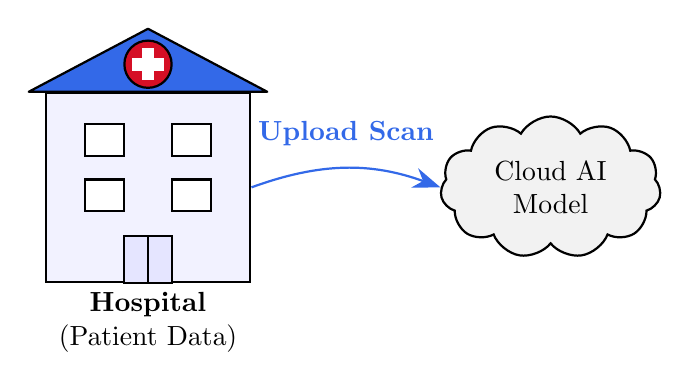
\begin{tikzpicture}
                % --- Szpital (Baza budynku) ---
                \node[draw, thick, fill=blue!5, minimum width=2.6cm, minimum height=2.4cm] (hospital) {};
                
                % Dach szpitala
                \draw[draw=black, thick, fill=myblue, line join=round] 
                    ($(hospital.north west) + (-0.2, 0)$) -- 
                    ($(hospital.north) + (0, 0.8)$) -- 
                    ($(hospital.north east) + (0.2, 0)$) -- cycle;
                    
                % Czerwone kółko i biały krzyż (na dachu)
                \fill[myred, draw=black, thick] ($(hospital.north) + (0, 0.35)$) circle (0.3cm);
                \fill[white] ($(hospital.north) + (-0.08, 0.15)$) rectangle ($(hospital.north) + (0.08, 0.55)$);
                \fill[white] ($(hospital.north) + (-0.2, 0.27)$) rectangle ($(hospital.north) + (0.2, 0.43)$);
                
                % Okna
                \fill[white, draw=black, thick] ($(hospital.center) + (-0.8, 0.4)$) rectangle ($(hospital.center) + (-0.3, 0.8)$);
                \fill[white, draw=black, thick] ($(hospital.center) + (0.3, 0.4)$) rectangle ($(hospital.center) + (0.8, 0.8)$);
                \fill[white, draw=black, thick] ($(hospital.center) + (-0.8, -0.3)$) rectangle ($(hospital.center) + (-0.3, 0.1)$);
                \fill[white, draw=black, thick] ($(hospital.center) + (0.3, -0.3)$) rectangle ($(hospital.center) + (0.8, 0.1)$);
                
                % Drzwi wejściowe
                \fill[blue!10, draw=black, thick] ($(hospital.south) + (-0.3, 0)$) rectangle ($(hospital.south) + (0.3, 0.6)$);
                \draw[thick] ($(hospital.south) + (0, 0)$) -- ($(hospital.south) + (0, 0.6)$); % linia podziału drzwi
                
                % Tekst pod budynkiem
                \node[align=center] at ($(hospital.south) - (0, 0.5)$) {\textbf{Hospital}\\(Patient Data)};
                
                % --- Chmura (odsunięta dalej) ---
                \node[cloud, cloud puffs=11, cloud puff arc=120, aspect=2, draw, thick, fill=gray!10, minimum width=2.8cm, minimum height=1.8cm, right=2.4cm of hospital, align=center] (cloud) {Cloud AI\\Model};
                
                % --- Strzałka z czytelnym tekstem ---
                \draw[-{Stealth[scale=1.5]}, thick, myblue] 
                    (hospital.east) to[out=20, in=160] 
                    node[midway, above, sloped, yshift=0.15cm] {\textbf{Upload Scan}} 
                    (cloud.west);
            \end{tikzpicture}
            }
        \end{column}
    \end{columns}
\end{frame}

% --- SLIDE 3: The Barrier ---
\begin{frame}{The Barrier: Strict Privacy Regulations}
    \begin{columns}
        \begin{column}{0.5\textwidth}
            \centering
            
\begin{tikzpicture}
                % Document
                \node[draw, thick, fill=white, minimum width=2cm, minimum height=2.5cm] (doc) {};
                \draw[thick] ($(doc.north west)+(0.3,-0.5)$) -- ($(doc.north east)+(-0.3,-0.5)$);
                \draw[thick] ($(doc.north west)+(0.3,-0.9)$) -- ($(doc.north east)+(-0.3,-0.9)$);
                \draw[thick] ($(doc.north west)+(0.3,-1.3)$) -- ($(doc.north east)+(-0.3,-1.3)$);
                % Lock
                \node[draw, thick, fill=myred!20, rounded corners, minimum width=1.2cm, minimum height=1cm, align=center, drop shadow] at (doc.center) {\textbf{GDPR} \\ \textbf{CCPA}};
                \draw[thick] ($(doc.center)+(-0.3, 0.5)$) arc[start angle=180, end angle=0, radius=0.3] -- ($(doc.center)+(0.3, 0.2)$);
            \end{tikzpicture}
        \end{column}
        
        \begin{column}{0.5\textwidth}
            \textbf{The Problem:}
            \begin{itemize}
                \item Clients cannot share sensitive healthcare records with untrusted cloud providers.
                \item Modern legislation (EU GDPR, California's CCPA) mandates strict data protection.
                \item \textbf{Conclusion:} Data MUST be encrypted before leaving the hospital. Plaintext transfer is illegal.
            \end{itemize}
        \end{column}
    \end{columns}
\end{frame}

% --- SLIDE 4: The Cloud Privacy Paradox (Part 1) ---
\begin{frame}{The Cloud Privacy Paradox}
    \textbf{The Dilemma:} If data must be encrypted (e.g., using standard AES), the cloud cannot access it to perform AI analysis.
    
    \vspace{0.8cm}
    \centering
    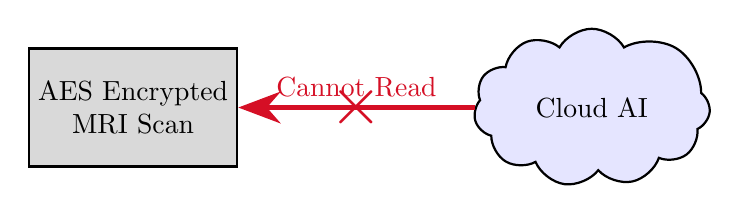
\begin{tikzpicture}
        % Encrypted Data
        \node[draw, thick, fill=gray!30, minimum width=2cm, minimum height=1.5cm, align=center] (aes) {AES Encrypted\\MRI Scan};
        % Cloud
        \node[cloud, cloud puffs=10.8, cloud puff arc=120, aspect=2, draw, thick, fill=blue!10, minimum width=3cm, minimum height=2cm, right=3cm of aes, align=center] (cloud) {Cloud AI};
        % Arrow with Cross
        \draw[-{Stealth[scale=1.5]}, ultra thick, myred] (cloud.west) -- node[midway, above] {Cannot Read} node[midway, align=center] {\Huge $\times$} (aes.east);
    \end{tikzpicture}
    
    \vspace{0.8cm}
    Traditional cryptography is designed \textbf{only for data confidentiality}, not for computation!
\end{frame}

% Slajd 1: Data Confidentiality (Teoria)
\begin{frame}{Traditional Cryptography: Data Confidentiality}
    \begin{block}{\faLock \ Data Confidentiality}
        The fundamental goal of hiding data from unauthorized parties. Typically achieved using symmetric encryption algorithms, such as the \textbf{AES (Advanced Encryption Standard)}.
    \end{block}
\end{frame}

% --- SLIDE 5: The Cloud Privacy Paradox (Part 2) ---
\begin{frame}{Naive Approach: Computing on AES Ciphertexts?}
    What if the cloud server simply tries to apply a mathematical filter directly to the encrypted AES bytes?
    \vspace{0.5cm}
    
    \begin{columns}
        \begin{column}{0.4\textwidth}
            \centering
            % Here you can normally put \includegraphics[width=\textwidth]{dog_corrupted.bmp}
            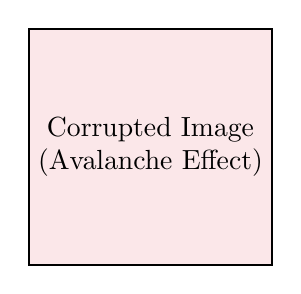
\begin{tikzpicture}
                \node[draw, thick, fill=myred!10, minimum width=3cm, minimum height=3cm, align=center] {Corrupted Image\\(Avalanche Effect)};
            \end{tikzpicture}
        \end{column}
        \begin{column}{0.6\textwidth}
            \textbf{The Avalanche Effect:}
            \begin{itemize}
                \item Modifying even a single byte of an AES ciphertext results in a destroyed plaintext.
                \item Any naive mathematical operation on ciphertext bytes irreversibly destroys the data.
            \end{itemize}
        \end{column}
    \end{columns}
\end{frame}

% Slajd 2: Data Confidentiality (Ilustracja AES)
%\begin{frame}{Traditional Cryptography: Symmetric Encryption Flow}    
%    \vspace{0.6cm}
%    \begin{center}
%    \resizebox{0.95\textwidth}{!}{%
%    \begin{tikzpicture}[
%        node distance=1.2cm and 1.2cm,
%        % Style poszczególnych elementów
%        plain/.style={draw=DeepBlue, thick, rectangle, minimum width=2.2cm, minimum height=1.2cm, align=center, fill=white, rounded corners, font=\small, drop shadow},
%        action/.style={draw=DeepBlue, thick, rectangle, minimum width=2.2cm, minimum height=1.2cm, align=center, fill=LightGray, rounded corners, font=\small, drop shadow},
%        data/.style={draw=AccentOrange, thick, rectangle, minimum width=2.2cm, minimum height=1.2cm, align=center, fill=AccentOrange!10, rounded corners, font=\small\bfseries, drop shadow},
%        key/.style={draw=red!70!black, thick, circle, minimum size=1.5cm, align=center, fill=red!10, font=\footnotesize, drop shadow},
%        % Style strzałek
%        arrow/.style={->, thick, DeepBlue, >=stealth},
%        keyarrow/.style={->, thick, dashed, red!70!black, >=stealth}
%    ]
%
%    % Węzły (Nodes)
%    \node (pt1) [plain] {\faFile \\ Plaintext\\(Sender)};
%    \node (enc) [action, right=of pt1] {\faLock \\ Encryption\\(AES)};
%    \node (ct)  [data, right=of enc] {\faMask \\ Ciphertext};
%    \node (dec) [action, right=of ct] {\faUnlock \\ Decryption\\(AES)};
%    \node (pt2) [plain, right=of dec] {\faFile \\ Plaintext\\(Receiver)};
%
%    % Klucz symetryczny
%    \node (key) [key, below=of ct, yshift=-0.5cm] {\faKey \\ Shared\\Secret};
%
%    % Strzałki przepływu danych
%    \draw [arrow] (pt1) -- (enc);
%    \draw [arrow] (enc) -- (ct);
%    \draw [arrow] (ct) -- (dec);
%    \draw [arrow] (dec) -- (pt2);
%
%    % Strzałki od klucza (przerywane)
%    \draw [keyarrow] (key) -| (enc);
%    \draw [keyarrow] (key) -| (dec);
%
%    \end{tikzpicture}%
%    }
%    \end{center}
%\end{frame}





\begin{frame}{Testing the Naive Approach: A Safe Experiment}
    \begin{columns}
        \begin{column}{0.5\textwidth}
            \textbf{The Naive Idea:}
            \begin{itemize}
                \item What if the cloud server simply ignores the encryption and applies a mathematical filter directly to the AES ciphertext bytes?
                \item Before we risk irreversibly destroying a patient's sensitive MRI scan, we must test this hypothesis safely.
            \end{itemize}
            \vspace{0.4cm}
            \textbf{Our Test Subject:}
            \begin{itemize}
                \item Instead of a medical record, let's use a harmless, standard image: \textbf{a photo of a Beagle dog}.
                \item We will ask the cloud to apply some changes to the encrypted dog photo. Let's see what happens...
            \end{itemize}
        \end{column}
        
        \begin{column}{0.5\textwidth}
            \centering
            % Resizebox chroni diagram przed wyjściem poza ekran
            \resizebox{0.8\textwidth}{!}{
            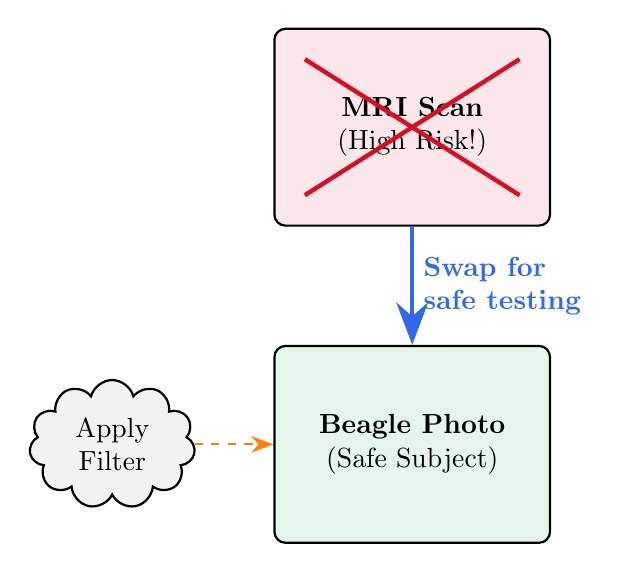
\begin{tikzpicture}
                % --- MRI Box ---
                \node[draw, thick, fill=myred!10, rounded corners, minimum width=3.5cm, minimum height=2.5cm, align=center] (mri) {\textbf{MRI Scan}\\(High Risk!)};
                
                % Czerwony krzyżyk na MRI
                \draw[ultra thick, myred] ($(mri.north west) + (0.4, -0.4)$) -- ($(mri.south east) + (-0.4, 0.4)$);
                \draw[ultra thick, myred] ($(mri.south west) + (0.4, 0.4)$) -- ($(mri.north east) + (-0.4, -0.4)$);
                
                % --- Strzałka w dół ---
                \draw[-{Stealth[scale=1.5]}, ultra thick, myblue] 
                    (mri.south) -- ++(0, -1.5cm) 
                    node[midway, right, align=left] {\textbf{Swap for}\\\textbf{safe testing}};
                    
                % --- Dog Box ---
                \node[draw, thick, fill=mygreen!10, rounded corners, minimum width=3.5cm, minimum height=2.5cm, align=center, below=1.5cm of mri] (dog) {\textbf{Beagle Photo}\\(Safe Subject)};
                
                % --- Mała chmurka z filtrem ---
                \node[cloud, cloud puffs=11, aspect=1.5, draw, thick, fill=gray!10, left=1cm of dog, align=center] (cloud) {Apply\\Filter};
                \draw[-{Stealth[scale=1.2]}, thick, dashed, orange] (cloud.east) -- (dog.west);
                
            \end{tikzpicture}
            }
        \end{column}
    \end{columns}
\end{frame}


% Slajd 3: The Fragility of Traditional Ciphers (Efekt Lawinowy na Bitmapie)
\begin{frame}{The Fragility of Traditional Ciphers (AES PCBC Mode)}
    \textbf{The Avalanche Effect:} Modifying the ciphertext destroys the decrypted data.
    
    \vspace{0.2cm}
    \begin{center}
        \begin{figure}
            \centering
            % Lewy obrazek - Oryginał
            \begin{minipage}{0.31\textwidth}
                \centering
                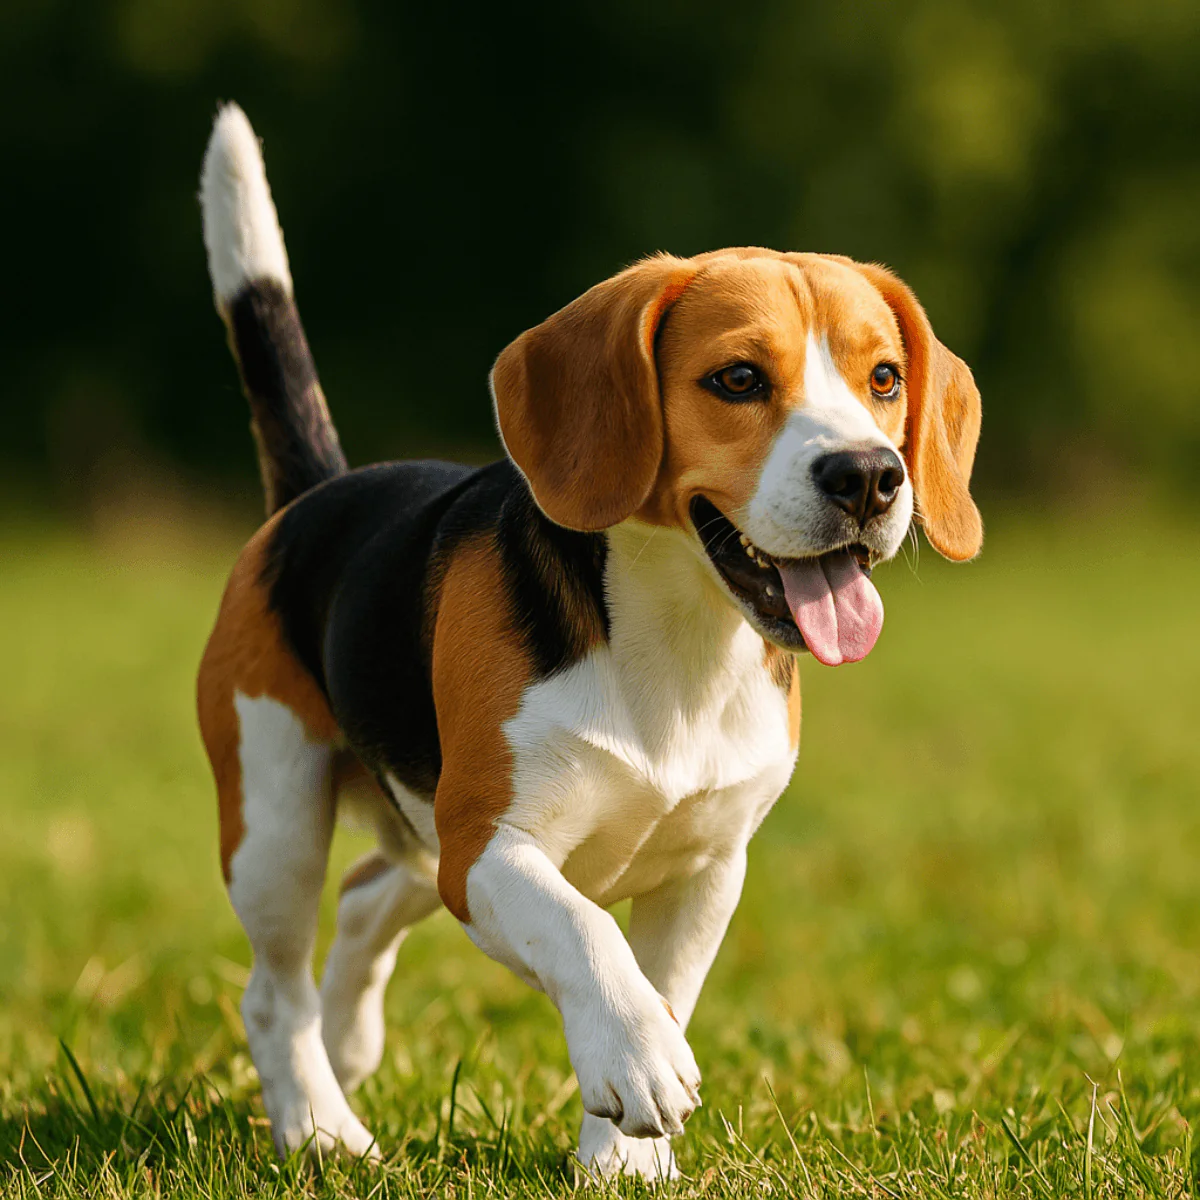
\includegraphics[width=\textwidth]{dog.png}
                \vspace{0.1cm}
                \textbf{dog.bmp}\\
                \footnotesize (Original)
            \end{minipage}\hfill
            % Strzałka i tekst pośrodku
            \begin{minipage}{0.38\textwidth}
                \centering
                \footnotesize \textbf{1 byte modified in ciphertext}\\
                \vspace{0.1cm}
                \scriptsize \textit{Corrupts one AES block (16 bytes)}\\
                \textit{propagates error to subsequent blocks}\\
                \textit{due to PCBC mode} \\
                \vspace{0.1cm}
                \Huge $\xrightarrow{\hspace*{1.5cm}}$
            \end{minipage}\hfill
            % Prawy obrazek - Zepsuty po deszyfrowaniu
            \begin{minipage}{0.31\textwidth}
                \centering
                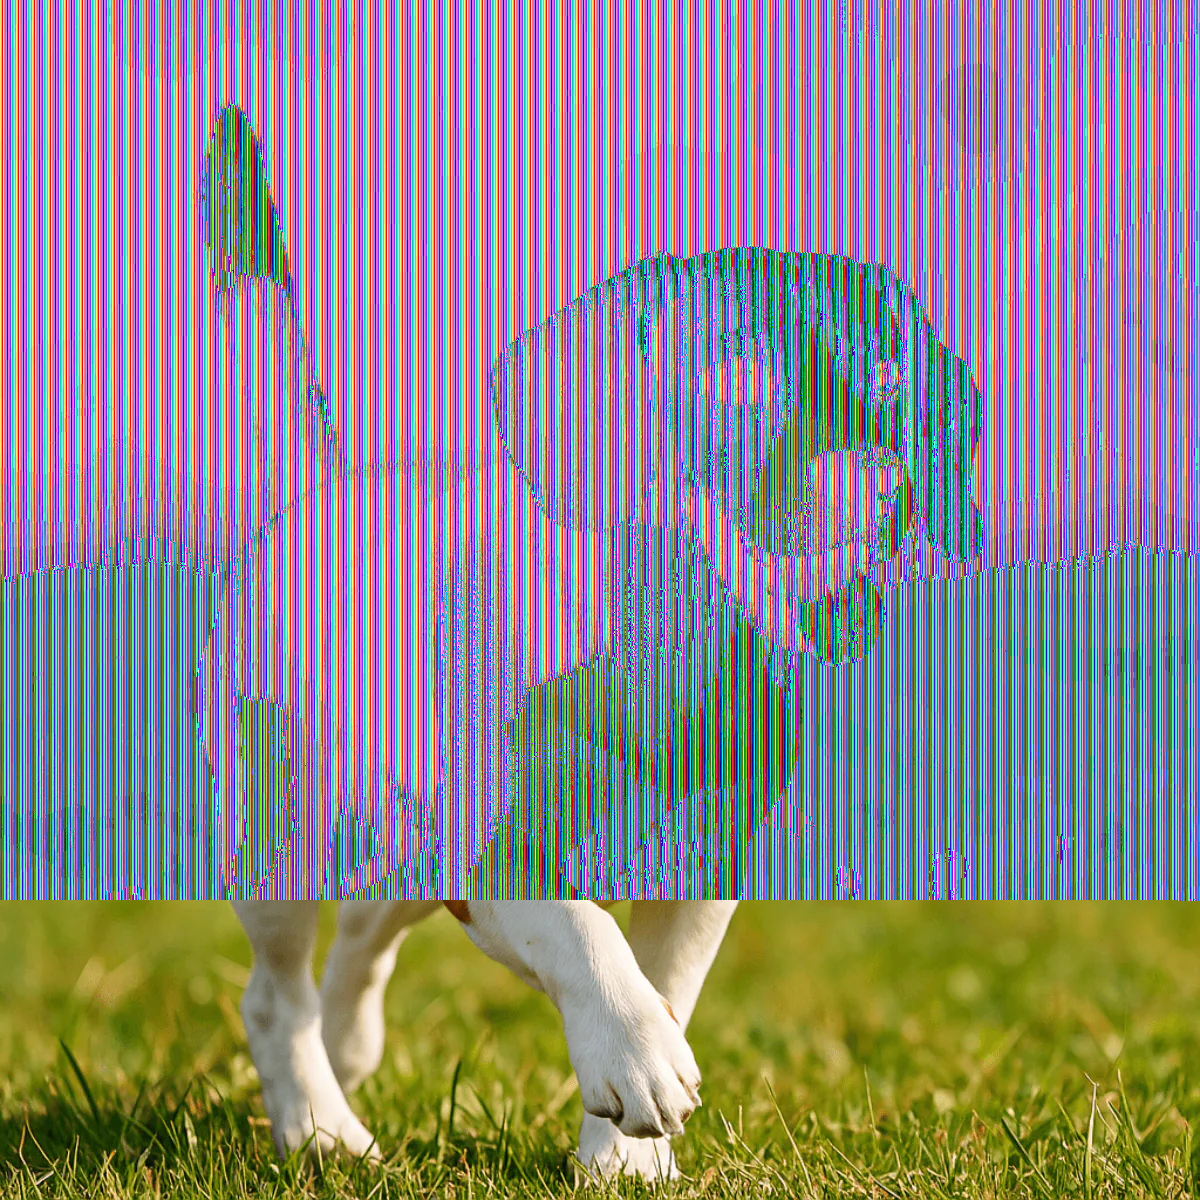
\includegraphics[width=\textwidth]{dog_corrupted.png}
                \vspace{0.1cm}
                \textbf{dog\_corrupted.bmp}\\
                \footnotesize (Decrypted)
            \end{minipage}
        \end{figure}
    \end{center}
\end{frame}

% Slajd 3: The Fragility of Traditional Ciphers (Efekt Lawinowy na Bitmapie)
\begin{frame}{The Fragility of Traditional Ciphers}
    \begin{alertblock}{\faExclamationTriangle \ The Avalanche Effect in AES}
        In traditional ciphers designed for confidentiality, \textbf{modifying the ciphertext destroys the underlying data}.
    \end{alertblock}
    
    \vspace{0.4cm}
    \begin{center}
    \resizebox{0.95\textwidth}{!}{%
    \begin{tikzpicture}[
        % Style kafelków
        plain/.style={draw=DeepBlue, thick, rectangle, minimum width=2.5cm, minimum height=1.2cm, align=center, fill=white, rounded corners, font=\small, drop shadow},
        action/.style={draw=DeepBlue, thick, rectangle, minimum width=2.5cm, minimum height=1.2cm, align=center, fill=LightGray, rounded corners, font=\small, drop shadow},
        data/.style={draw=AccentOrange, thick, rectangle, minimum width=2.5cm, minimum height=1.2cm, align=center, fill=AccentOrange!10, rounded corners, font=\small\bfseries, drop shadow},
        corrupted/.style={draw=red!70!black, thick, rectangle, minimum width=2.5cm, minimum height=1.2cm, align=center, fill=red!10, rounded corners, font=\small\bfseries, drop shadow},
        % Style strzałek
        arrow/.style={->, thick, DeepBlue, >=stealth},
        attackarrow/.style={->, thick, dashed, red!70!black, >=stealth}
    ]

    % Górny rząd (Prawidłowy przepływ)
    \node (img_orig) at (0, 0) [plain] {\faImage \\ Original Bitmap\\(Plaintext)};
    \node (enc1) at (3.8, 0) [action] {\faLock \\ Encrypt (AES)};
    \node (ct1) at (7.6, 0) [data] {\faMask \\ Ciphertext};
    \node (dec1) at (11.4, 0) [action] {\faUnlock \\ Decrypt (AES)};
    \node (img_dec) at (15.2, 0) [plain, draw=green!60!black] {\textcolor{green!60!black}{\faCheckCircle} \\ Perfect Bitmap\\(Plaintext)};

    \draw [arrow] (img_orig) -- (enc1);
    \draw [arrow] (enc1) -- (ct1);
    \draw [arrow] (ct1) -- (dec1);
    \draw [arrow] (dec1) -- (img_dec);

    % Dolny rząd (Zmodyfikowany przepływ - Atak)
    \node (ct2) at (7.6, -3) [corrupted] {\faBug \\ Modified Ciphertext\\(1 byte flipped)};
    \node (dec2) at (11.4, -3) [action] {\faUnlock \\ Decrypt (AES)};
    \node (img_corr) at (15.2, -3) [corrupted] {\faSkullCrossbones \\ Corrupted Bitmap\\(Invalid plaintext)};

    % Strzałka z modyfikacją
    \draw [attackarrow] (ct1) -- node[right, align=center, font=\footnotesize, text=red!70!black] {Attacker flips\\a single byte} (ct2);
    \draw [arrow] (ct2) -- (dec2);
    \draw [arrow] (dec2) -- (img_corr);

    \end{tikzpicture}%
    }
    \end{center}
\end{frame}

% Slajd 4: The Motivation for FHE (Zapotrzebowanie na modyfikacje)
\begin{frame}{The Goal: Computing on Encrypted Data}
    \begin{columns}
        % Lewa kolumna: Tekst i problem
        \begin{column}{0.55\textwidth}            
            For simplicity, let's say the modification is a basic filter: \textbf{making the center of the photo grayscale}.
            
            \vspace{0.4cm}
            \begin{alertblock}{The Problem}
                How do we build such a service?\\
                As we just saw, if we try to modify \textbf{AES ciphertexts}, we will destroy the image!
            \end{alertblock}
        \end{column}
        
        % Prawa kolumna: Zdjęcie
        \begin{column}{0.40\textwidth}
            \begin{figure}
                \centering
                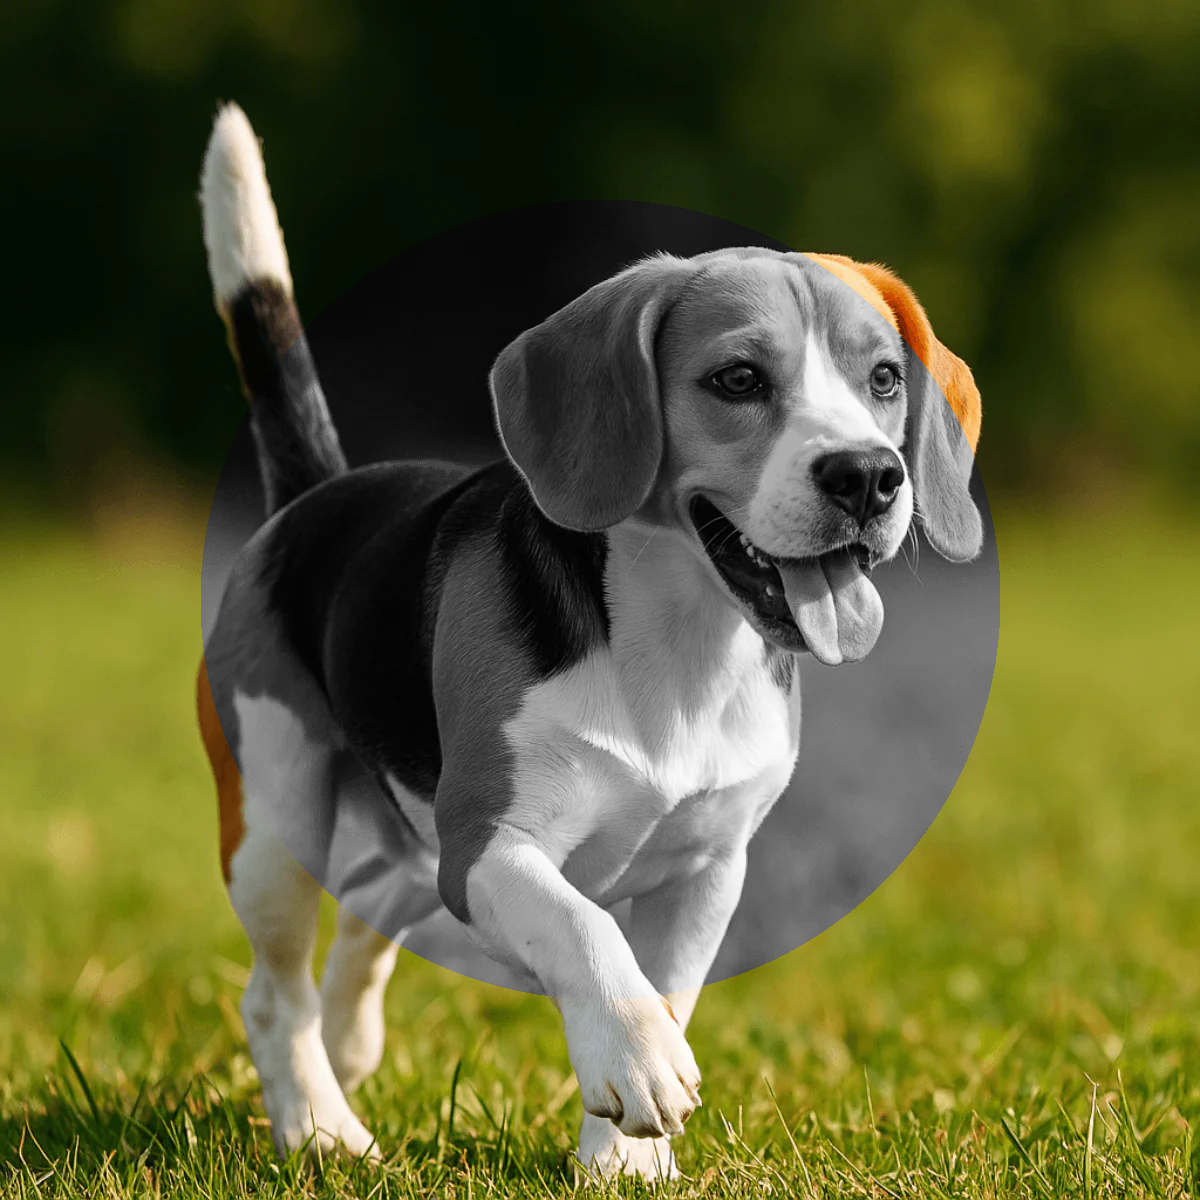
\includegraphics[width=0.95\textwidth]{dog_with_circle.png}
                \vspace{0.1cm}
                \\ \footnotesize \textbf{Desired Output}
            \end{figure}
        \end{column}
    \end{columns}
\end{frame}

% Slajd 5: Naiwne podejście - modyfikacja szyfrogramu
\begin{frame}{Naive Approach: Modifying the Ciphertext}
    \begin{columns}
        % Lewa kolumna: Tekst i wyjaśnienie
        \begin{column}{0.55\textwidth}
            \textbf{The Naive Attempt:}\\
            What if the cloud server simply applies the grayscale filter directly to the \textit{encrypted} pixels?
            
            \vspace{0.4cm}
            \textbf{The Result:}\\
            Because of the \textbf{Avalanche Effect}, any mathematical operation on the ciphertext bytes irreversibly destroys the data. Even in ECB mode (Electronic Codebook), used here to limit error propagation.
            
            \vspace{0.4cm}
            \begin{alertblock}{Decryption Failure}
                Instead of a grayscale center, the user decrypts a completely corrupted hole of random noise!
            \end{alertblock}
        \end{column}
        
        % Prawa kolumna: Zdjęcie zepsutego psa
        \begin{column}{0.40\textwidth}
            \begin{figure}
                \centering
                % Pamiętaj o użyciu wersji .png dla kompilatora pdflatex
                
\includegraphics[width=0.95\textwidth]{dog_cipher_grayscale.png}
                \vspace{0.1cm}
                \\ \footnotesize \textbf{Decrypted Result}
            \end{figure}
        \end{column}
    \end{columns}
\end{frame}

% Slajd 6a: Czym jest FHE (Definicja)
\begin{frame}{The Solution: Fully Homomorphic Encryption (FHE)}
    \textbf{The Challenge Resolved:} What if we \textit{want} to modify the ciphertext in a meaningful way to perform computations without decrypting it?
    
    \vspace{0.5cm}
    \begin{block}{What is FHE?}
        \textbf{Fully Homomorphic Encryption (FHE)} is a cryptographic scheme that enables computations to be performed directly on encrypted data, as if the data were in plaintext.
    \end{block}
    
    \vspace{0.5cm}
    Unlike traditional ciphers, FHE allows the cloud server to apply our grayscale filter directly to the encrypted bytes without ever seeing the original photo.
\end{frame}

\begin{frame}{FHE in Action: Secure Cloud Filtering}
    \begin{center}
    \resizebox{0.95\textwidth}{!}{%
    \begin{tikzpicture}[
        box/.style={draw=DeepBlue, thick, rectangle, minimum width=1.5cm, minimum height=0.6cm, align=center, fill=LightGray, rounded corners, font=\scriptsize, drop shadow},
        data/.style={draw=AccentOrange, thick, rectangle, minimum width=1.6cm, minimum height=0.6cm, align=center, fill=AccentOrange!10, rounded corners, font=\scriptsize, drop shadow},
        cloud/.style={draw=DeepBlue!50, rectangle, rounded corners=10pt, minimum width=2.5cm, minimum height=1.2cm, fill=DeepBlue!5, align=center, thick, dashed, font=\scriptsize},
        arrow/.style={->, thick, DeepBlue, >=stealth}
    ]

    % STREFY
    \node at (1.2, 1.2) [font=\small\bfseries, color=DeepBlue] {\faUser \ Client};
    \node at (7.5, 1.2) [font=\small\bfseries, color=gray!80!black] {\faCloud \ Cloud Service};
    
    \draw[dashed, gray!50, thick] (3.8, 1.4) -- (3.8, -3.2);

    % KLIENT (Szyfrowanie)
    \node (img_in) at (0, 0) {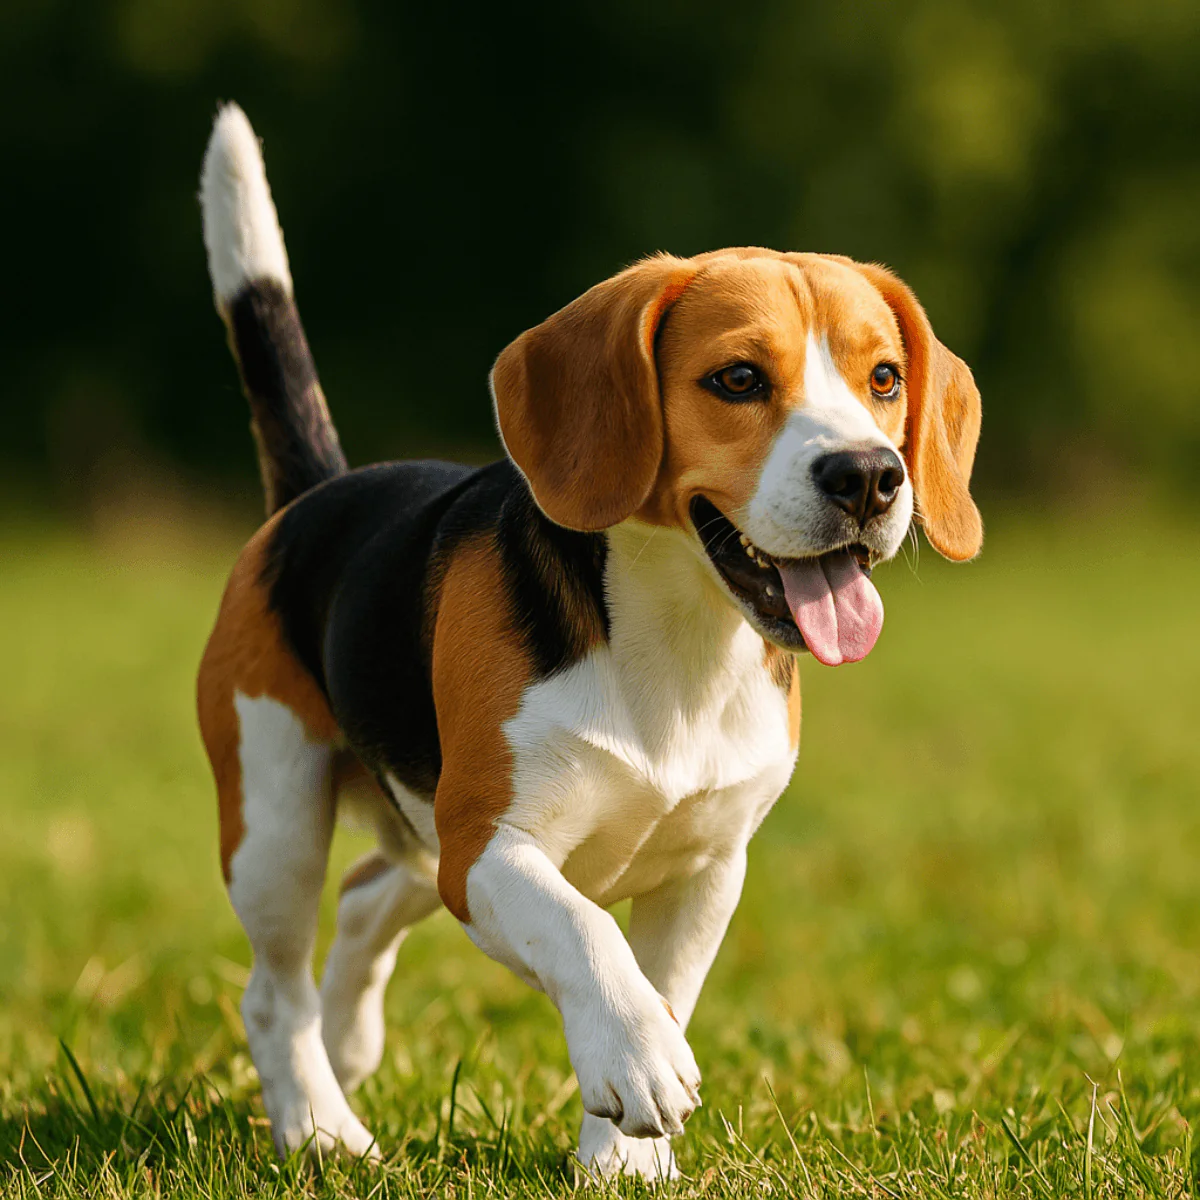
\includegraphics[width=1cm]{dog.png}};
    \node (enc) at (2.2, 0) [box, fill=green!10, draw=green!60!black] {\faLock \\ Encrypt (FHE)};
    \draw [arrow] (img_in) -- (enc);

    % WYSYŁKA
    \node (ct_in) at (4.8, 0) [data] {\\ Ciphertext};
    \draw [arrow] (enc) -- (ct_in);

    % CHMURA
    \node (cloud) at (7.8, -1) [cloud] {\textbf{\faCogs \ Homomorphic}\\\textbf{Evaluation}\\[0.1cm]Apply Filter};
    \draw [arrow] (ct_in.east) -| (cloud.north);

    % ODBIÓR
    \node (ct_out) at (4.8, -2) [data] {\\ Modified\\Ciphertext};
    \draw [arrow] (cloud.south) |- (ct_out.east);

    % KLIENT (Deszyfrowanie)
    \node (dec) at (2.2, -2) [box, fill=green!10, draw=green!60!black] {\faUnlock \\ Decrypt (FHE)};
    \node (img_out) at (0, -2) {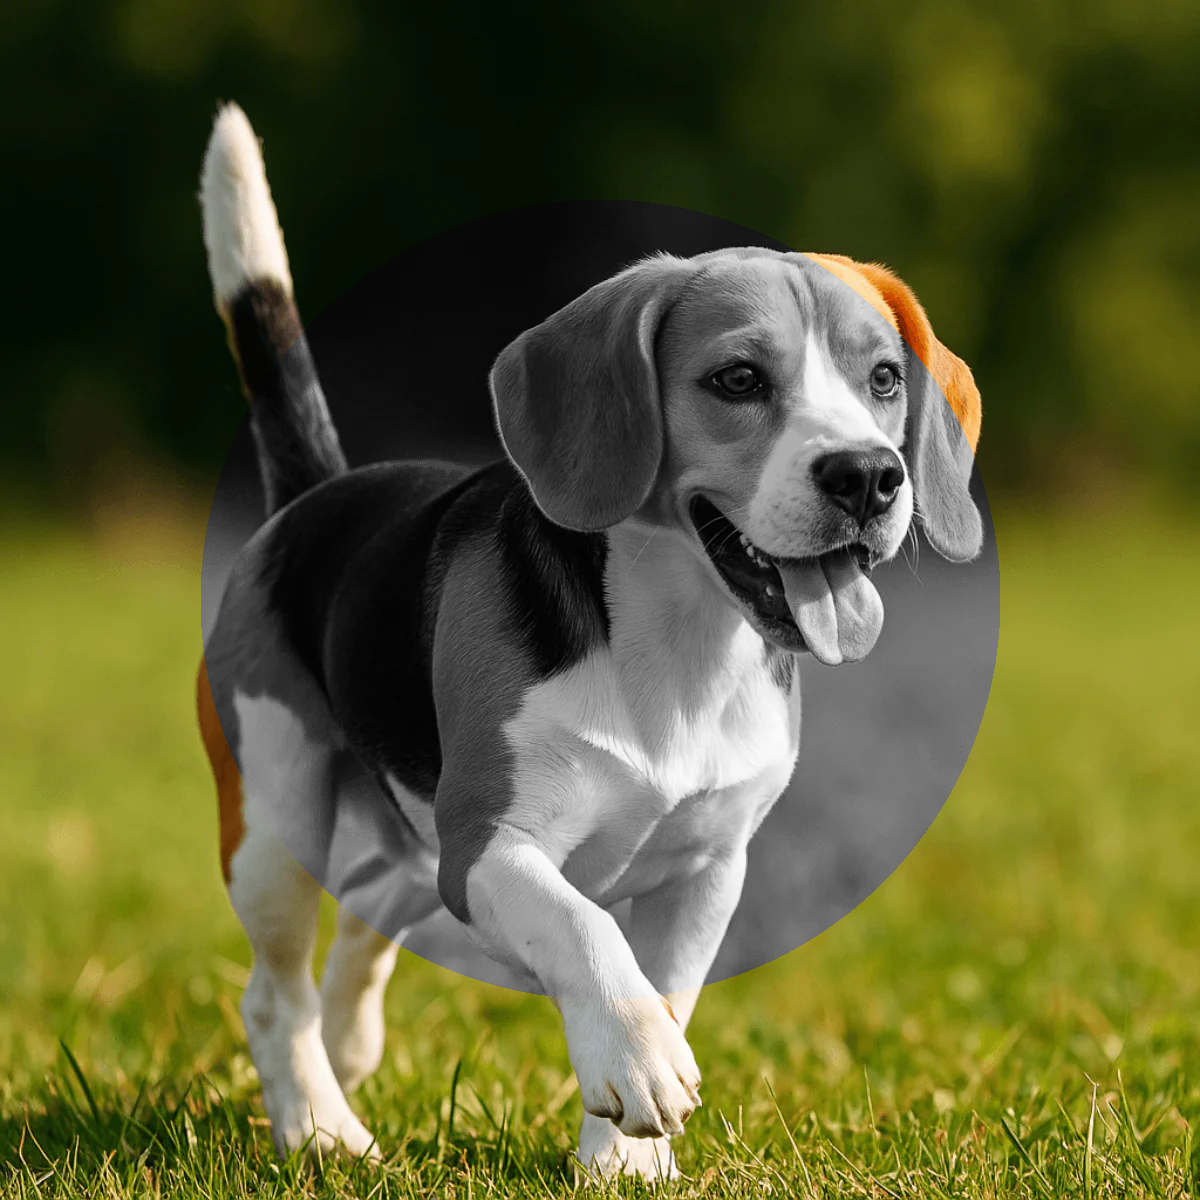
\includegraphics[width=1cm]{dog_with_circle.png}};
    
    \draw [arrow] (ct_out) -- (dec);
    \draw [arrow] (dec) -- (img_out);

    \end{tikzpicture}%
    }
    \end{center}
\end{frame}
% Slajd 6b: Zastosowania FHE
\begin{frame}{Key Applications of FHE}
    Because FHE allows computations on hidden data, it unlocks entirely new paradigms for data security:
    \vspace{0.4cm}
    
    \begin{itemize}
        \item[\faCloud] \textbf{Privacy-Preserving Cloud Computing:} Secure outsourcing of data analytics and encrypted database queries to untrusted cloud servers.
        \vspace{0.3cm}
        \item[\faRobot] \textbf{Secure Machine Learning:} Allowing a server to process a client's encrypted data through an ML model without exposing the input features or the inference results.
        \vspace{0.3cm}
        \item[\faLink] \textbf{Confidential Blockchain Services:} Ensuring that sensitive data in smart contracts remains encrypted and confidential while maintaining execution transparency.
    \end{itemize}
\end{frame}

% --- SLIDE 8: Another Goal ---
\begin{frame}{Another Application: Secure Digital Voting}
    \begin{columns}
        \begin{column}{0.5\textwidth}
            \textbf{Scenario:}
            \begin{itemize}
                \item We want to build a fully secure, remote digital voting system for national elections.
                \item Every citizen submits their ballot electronically.
            \end{itemize}
            \vspace{0.5cm}
            \textbf{Value:} Maximum convenience and high voter turnout, but it requires absolute mathematical trust in the election integrity.
        \end{column}
        
        \begin{column}{0.5\textwidth}
            \centering
            \resizebox{0.9\textwidth}{!}{
            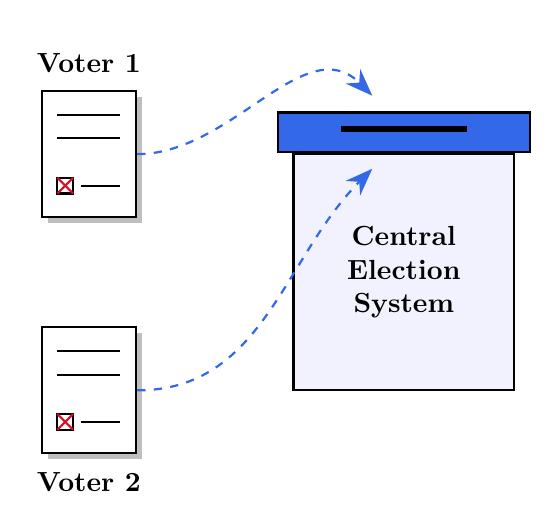
\begin{tikzpicture}
                % --- Digital Ballot Box (Urna) ---
                \node[draw=black, thick, fill=blue!5, minimum width=2.8cm, minimum height=3cm] (box) at (4,0) {};
                \node[draw=black, thick, fill=myblue, minimum width=3.2cm, minimum height=0.5cm, anchor=south] (lid) at (box.north) {};
                \fill[black] ($(lid.center)+(-0.8, 0)$) rectangle ($(lid.center)+(0.8, 0.08)$); % Szczelina
                \node[align=center] at (box.center) {\textbf{Central}\\\textbf{Election}\\\textbf{System}};
                
                % --- Voter 1 Ballot (Wyprostowana) ---
                \begin{scope}[shift={(0, 1.5)}]
                    \node[draw=black, thick, fill=white, minimum width=1.2cm, minimum height=1.6cm, drop shadow] (b1) at (0,0) {};
                    \draw[thick] (-0.4, 0.5) -- (0.4, 0.5);
                    \draw[thick] (-0.4, 0.2) -- (0.4, 0.2);
                    % Checkbox i krzyżyk
                    \draw[thick] (-0.4, -0.3) rectangle (-0.2, -0.5);
                    \draw[thick, myred] (-0.4, -0.3) -- (-0.2, -0.5);
                    \draw[thick, myred] (-0.4, -0.5) -- (-0.2, -0.3);
                    \draw[thick] (-0.1, -0.4) -- (0.4, -0.4);
                \end{scope}
                \node[above=0.1cm of b1] {\textbf{Voter 1}};

                % --- Voter 2 Ballot (Wyprostowana) ---
                \begin{scope}[shift={(0, -1.5)}]
                    \node[draw=black, thick, fill=white, minimum width=1.2cm, minimum height=1.6cm, drop shadow] (b2) at (0,0) {};
                    \draw[thick] (-0.4, 0.5) -- (0.4, 0.5);
                    \draw[thick] (-0.4, 0.2) -- (0.4, 0.2);
                    % Checkbox i krzyżyk
                    \draw[thick] (-0.4, -0.3) rectangle (-0.2, -0.5);
                    \draw[thick, myred] (-0.4, -0.3) -- (-0.2, -0.5);
                    \draw[thick, myred] (-0.4, -0.5) -- (-0.2, -0.3);
                    \draw[thick] (-0.1, -0.4) -- (0.4, -0.4);
                \end{scope}
                \node[below=0.1cm of b2] {\textbf{Voter 2}};

                % --- Krzywe strzałki wpadające do urny ---
                \draw[-{Stealth[scale=1.5]}, thick, myblue, dashed] (b1.east) to[out=0, in=135] ($(lid.north)+(-0.4, 0.2)$);
                \draw[-{Stealth[scale=1.5]}, thick, myblue, dashed] (b2.east) to[out=0, in=225] ($(lid.south)+(-0.4, -0.2)$);
            \end{tikzpicture}
            }
        \end{column}
    \end{columns}
\end{frame}

% --- SLIDE 9: The Voting Dilemma ---
\begin{frame}{The Voting Dilemma: Privacy vs. Verifiability}
    \begin{columns} % Usunięto [T], by tekst wyśrodkował się naturalnie względem obrazka
        \begin{column}{0.4\textwidth}
            \centering
            % Kolejne zmniejszenie rysunku (z 0.55 na 0.45)
            \resizebox{0.45\textwidth}{!}{
            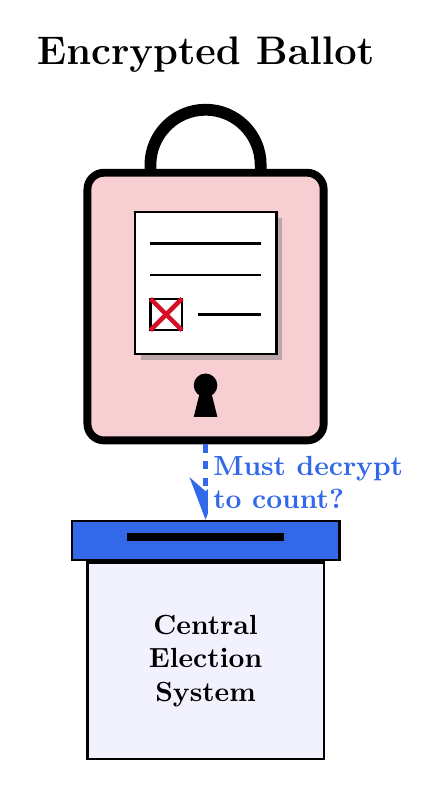
\begin{tikzpicture}
                % --- Server / Ballot Box (Kolor zmieniony na blue!5 jak w Slajdzie 8) ---
                \node[draw=black, thick, fill=blue!5, minimum width=3cm, minimum height=2.5cm] (server) at (0,-2.5) {};
                \node[draw=black, thick, fill=myblue, minimum width=3.4cm, minimum height=0.5cm, anchor=south] (lid) at (server.north) {};
                \fill[black] ($(lid.center)+(-1, 0)$) rectangle ($(lid.center)+(1, 0.1)$); % Szczelina
                \node[align=center] at (server.center) {\textbf{Central }\\\textbf{Election}\\\textbf{System}};
                
                % --- Encrypted Ballot (Realistyczna kłódka z kartą wewnątrz) ---
                \begin{scope}[shift={(0, 2)}]
                    % Pałąk kłódki
                    \draw[line width=1.5mm, draw=black] (-0.7, 1.2) -- (-0.7, 1.8) arc[start angle=180, end angle=0, radius=0.7] -- (0.7, 1.2);
                    
                    % Korpus kłódki
                    \node[draw=black, line width=1mm, fill=myred!20, rounded corners=6pt, minimum width=3cm, minimum height=3.4cm] (lock) at (0,0) {};
                    
                    % Wewnętrzna karta do głosowania
                    \node[draw=black, thick, fill=white, minimum width=1.8cm, minimum height=1.8cm, drop shadow] (paper) at (0, 0.3) {};
                    \draw[thick] (-0.7, 0.8) -- (0.7, 0.8);
                    \draw[thick] (-0.7, 0.4) -- (0.7, 0.4);
                    
                    % Checkbox i krzyżyk (przesunięte wyżej)
                    \draw[thick] (-0.7, 0.1) rectangle (-0.3, -0.3);
                    \draw[ultra thick, myred] (-0.7, 0.1) -- (-0.3, -0.3);
                    \draw[ultra thick, myred] (-0.7, -0.3) -- (-0.3, 0.1);
                    \draw[thick] (-0.1, -0.1) -- (0.7, -0.1);

                    % Dziurka od klucza (Keyhole)
                    \fill[black] (0, -1) circle (0.15cm);
                    \fill[black] (-0.15, -1.4) -- (0.15, -1.4) -- (0.05, -1) -- (-0.05, -1) -- cycle;
                    
                    % Podpis nad kłódką (umieszczony sztywno i wysoko, by omijał pałąk)
                    \node[font=\Large] at (0, 3.2) {\textbf{Encrypted Ballot}};
                \end{scope}
                
                % --- Arrow and Dilemma ---
                \draw[-{Stealth[scale=1.5]}, ultra thick, myblue, dashed] (lock.south) -- node[midway, right, align=left, font=\bfseries, fill=white, inner sep=2pt] {Must decrypt\\to count?} (lid.north);
            \end{tikzpicture}
            }
        \end{column}
        
        \begin{column}{0.6\textwidth}
            % Usunięto sztuczne przesuwanie tekstu w górę
            \textbf{The Problem:}
            \begin{itemize}
                \item To ensure voter privacy, ballots must be strictly encrypted before leaving the device.
                \item However, to tally the results, a standard cryptographic system (like AES) requires the central server to \textbf{decrypt} the votes first.
                \item \textbf{Privacy Compromised:} The system admin or a hacker could see exactly how every individual voted!
            \end{itemize}
        \end{column}
    \end{columns}
\end{frame}

% --- SLIDE 10: FHE Homomorphic Addition ---
\begin{frame}{The FHE Solution: Homomorphic Addition}
    \textbf{Fully Homomorphic Encryption} allows the server to mathematically tally the results while the votes remain completely encrypted!
    
    \vspace{0.6cm}
    \centering
    % Resizebox dba o to, by długie równanie graficzne zmieściło się w oknie
    \resizebox{0.95\textwidth}{!}{
    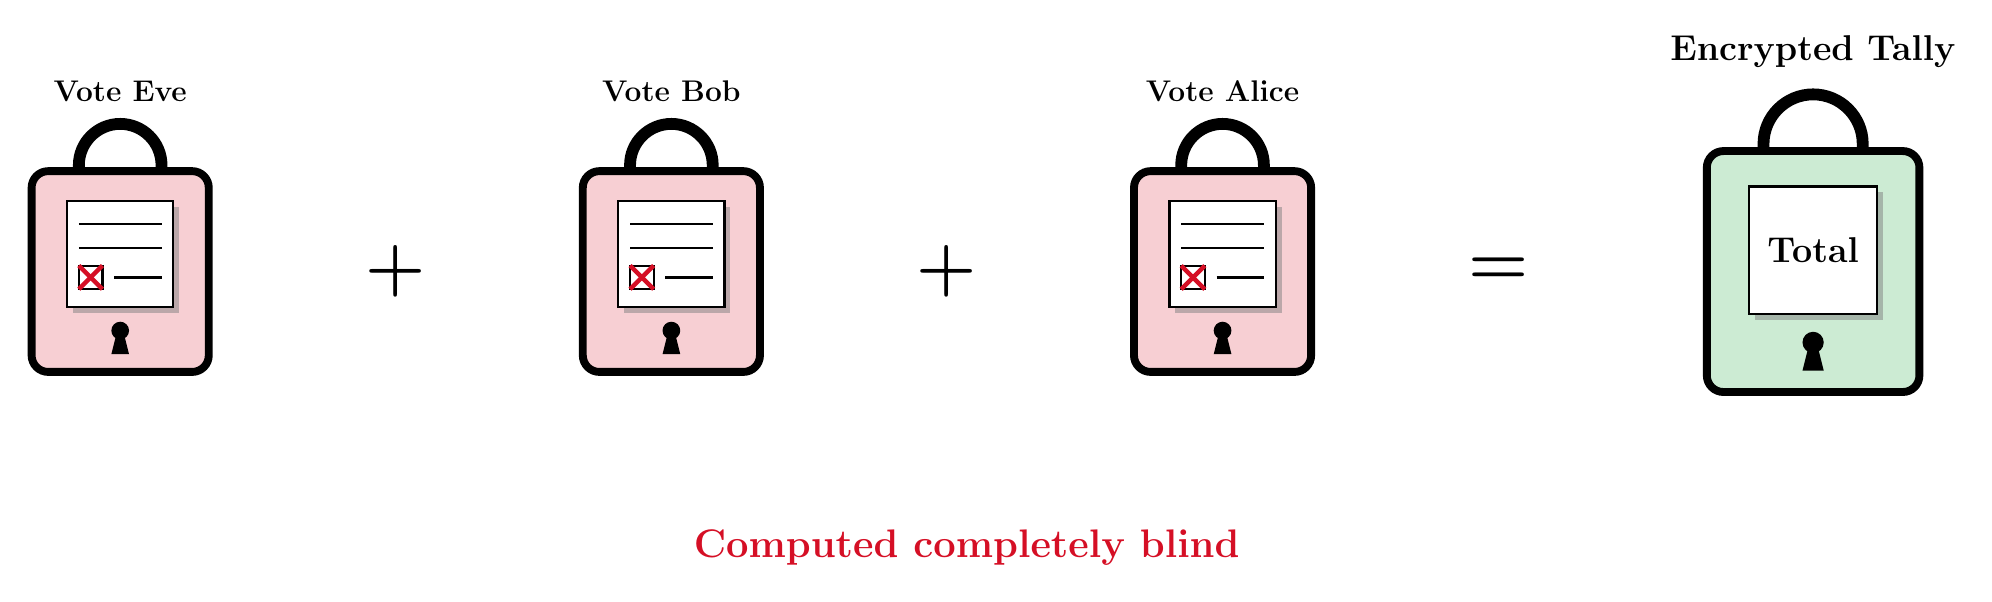
\begin{tikzpicture}
        % --- Encrypted Vote 1 (Alice) ---
        \begin{scope}[shift={(0,0)}, scale=0.75, transform shape]
            % Pałąk kłódki
            \draw[line width=1.5mm, draw=black] (-0.7, 1.2) -- (-0.7, 1.8) arc[start angle=180, end angle=0, radius=0.7] -- (0.7, 1.2);
            % Korpus kłódki
            \node[draw=black, line width=1mm, fill=myred!20, rounded corners=6pt, minimum width=3cm, minimum height=3.4cm] (lock1) at (0,0) {};
            % Wewnętrzna karta do głosowania
            \node[draw=black, thick, fill=white, minimum width=1.8cm, minimum height=1.8cm, drop shadow] (paper1) at (0, 0.3) {};
            \draw[thick] (-0.7, 0.8) -- (0.7, 0.8);
            \draw[thick] (-0.7, 0.4) -- (0.7, 0.4);
            % Checkbox i krzyżyk
            \draw[thick] (-0.7, 0.1) rectangle (-0.3, -0.3);
            \draw[ultra thick, myred] (-0.7, 0.1) -- (-0.3, -0.3);
            \draw[ultra thick, myred] (-0.7, -0.3) -- (-0.3, 0.1);
            \draw[thick] (-0.1, -0.1) -- (0.7, -0.1);
            % Dziurka od klucza
            \fill[black] (0, -1) circle (0.15cm);
            \fill[black] (-0.15, -1.4) -- (0.15, -1.4) -- (0.05, -1) -- (-0.05, -1) -- cycle;
            % Podpis (przesunięty wyżej)
            \node[above=1cm of lock1, font=\Large] {\textbf{Vote Eve}};
        \end{scope}
        
        % Plus
        \node at (3.5, 0) {\Huge \textbf{+}};
        
        % --- Encrypted Vote 2 (Bob) ---
        \begin{scope}[shift={(7,0)}, scale=0.75, transform shape]
            \draw[line width=1.5mm, draw=black] (-0.7, 1.2) -- (-0.7, 1.8) arc[start angle=180, end angle=0, radius=0.7] -- (0.7, 1.2);
            \node[draw=black, line width=1mm, fill=myred!20, rounded corners=6pt, minimum width=3cm, minimum height=3.4cm] (lock2) at (0,0) {};
            \node[draw=black, thick, fill=white, minimum width=1.8cm, minimum height=1.8cm, drop shadow] (paper2) at (0, 0.3) {};
            \draw[thick] (-0.7, 0.8) -- (0.7, 0.8);
            \draw[thick] (-0.7, 0.4) -- (0.7, 0.4);
            \draw[thick] (-0.7, 0.1) rectangle (-0.3, -0.3);
            \draw[ultra thick, myred] (-0.7, 0.1) -- (-0.3, -0.3);
            \draw[ultra thick, myred] (-0.7, -0.3) -- (-0.3, 0.1);
            \draw[thick] (-0.1, -0.1) -- (0.7, -0.1);
            \fill[black] (0, -1) circle (0.15cm);
            \fill[black] (-0.15, -1.4) -- (0.15, -1.4) -- (0.05, -1) -- (-0.05, -1) -- cycle;
            \node[above=1cm of lock2, font=\Large] {\textbf{Vote Bob}};
        \end{scope}
        
        % Plus
        \node at (10.5, 0) {\Huge \textbf{+}};
        
        % --- Encrypted Vote 3 (Alice) ---
        \begin{scope}[shift={(14,0)}, scale=0.75, transform shape]
            \draw[line width=1.5mm, draw=black] (-0.7, 1.2) -- (-0.7, 1.8) arc[start angle=180, end angle=0, radius=0.7] -- (0.7, 1.2);
            \node[draw=black, line width=1mm, fill=myred!20, rounded corners=6pt, minimum width=3cm, minimum height=3.4cm] (lock3) at (0,0) {};
            \node[draw=black, thick, fill=white, minimum width=1.8cm, minimum height=1.8cm, drop shadow] (paper3) at (0, 0.3) {};
            \draw[thick] (-0.7, 0.8) -- (0.7, 0.8);
            \draw[thick] (-0.7, 0.4) -- (0.7, 0.4);
            \draw[thick] (-0.7, 0.1) rectangle (-0.3, -0.3);
            \draw[ultra thick, myred] (-0.7, 0.1) -- (-0.3, -0.3);
            \draw[ultra thick, myred] (-0.7, -0.3) -- (-0.3, 0.1);
            \draw[thick] (-0.1, -0.1) -- (0.7, -0.1);
            \fill[black] (0, -1) circle (0.15cm);
            \fill[black] (-0.15, -1.4) -- (0.15, -1.4) -- (0.05, -1) -- (-0.05, -1) -- cycle;
            \node[above=1cm of lock3, font=\Large] {\textbf{Vote Alice}};
        \end{scope}
        
        % Equals
        \node at (17.5, 0) {\Huge \textbf{=}};
        
        % --- Encrypted Tally (Większa zielona kłódka z wynikiem) ---
        \begin{scope}[shift={(21.5,0)}, scale=0.9, transform shape]
            \draw[line width=1.5mm, draw=black] (-0.7, 1.2) -- (-0.7, 1.8) arc[start angle=180, end angle=0, radius=0.7] -- (0.7, 1.2);
            \node[draw=black, line width=1mm, fill=mygreen!20, rounded corners=6pt, minimum width=3cm, minimum height=3.4cm] (lock4) at (0,0) {};
            \node[draw=black, thick, fill=white, minimum width=1.8cm, minimum height=1.8cm, drop shadow, align=center] (paper4) at (0, 0.3) {\Large \textbf{Total}};
            \fill[black] (0, -1) circle (0.15cm);
            \fill[black] (-0.15, -1.4) -- (0.15, -1.4) -- (0.05, -1) -- (-0.05, -1) -- cycle;
            \node[above=1cm of lock4, font=\Large] {\textbf{Encrypted Tally}};
        \end{scope}
        
        % --- Label below ---
        % Wyrównane idealnie do środka w poziomie względem całego równania (10.75 to punkt na osi X dokładnie pomiędzy Vote 1 a Tally)
        \node[myred, font=\Large\bfseries] at (10.75, -3.5) {Computed completely blind};
    \end{tikzpicture}
    }
\end{frame}

% --- SLIDE 11: FHE Election Integrity ---
\begin{frame}{Absolute Election Integrity}
    \begin{columns}
        \begin{column}{0.25\textwidth}
            \centering
            \resizebox{0.95\textwidth}{!}{
            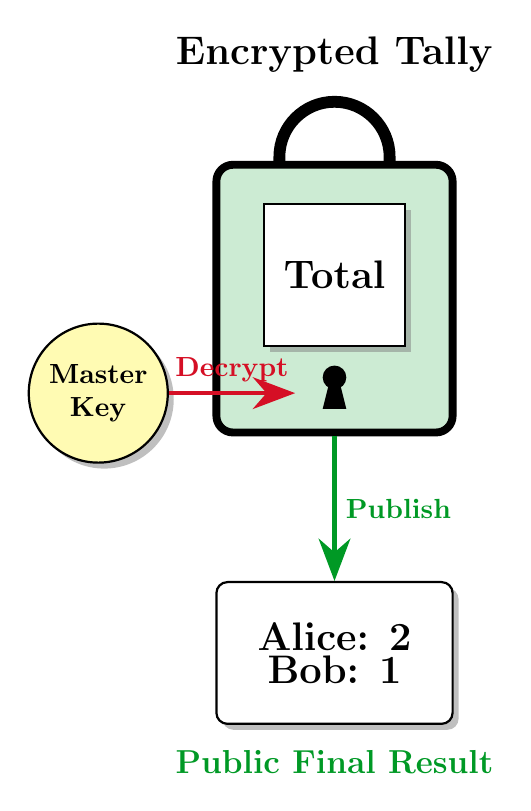
\begin{tikzpicture}
                % --- Encrypted Final Tally (Zielona kłódka z poprzedniego slajdu) ---
                \begin{scope}[shift={(0, 2)}]
                    % Pałąk kłódki
                    \draw[line width=1.5mm, draw=black] (-0.7, 1.2) -- (-0.7, 1.8) arc[start angle=180, end angle=0, radius=0.7] -- (0.7, 1.2);
                    
                    % Korpus kłódki
                    \node[draw=black, line width=1mm, fill=mygreen!20, rounded corners=6pt, minimum width=3cm, minimum height=3.4cm] (lock) at (0,0) {};
                    
                    % Wewnętrzna karta (Total)
                    \node[draw=black, thick, fill=white, minimum width=1.8cm, minimum height=1.8cm, drop shadow, align=center] (paper) at (0, 0.3) {\Large \textbf{Total}};
                    
                    % Dziurka od klucza
                    \fill[black] (0, -1) circle (0.15cm);
                    \fill[black] (-0.15, -1.4) -- (0.15, -1.4) -- (0.05, -1) -- (-0.05, -1) -- cycle;
                    
                    % Podpis nad kłódką
                    \node[above=1cm of lock, font=\Large] {\textbf{Encrypted Tally}};
                \end{scope}
                
                % --- Master Key ---
                % Klucz po lewej stronie, celujący prosto w dziurkę od klucza
                \node[draw=black, thick, fill=yellow!30, circle, minimum size=1.5cm, align=center, drop shadow] (key) at (-3, 0.8) {\textbf{Master}\\\textbf{Key}};
                
                % Strzałka od klucza do kłódki
                \draw[-{Stealth[scale=1.5]}, ultra thick, myred] (key.east) -- node[midway, above, font=\bfseries] {Decrypt} (-0.5, 0.8);
                
                % --- Decrypted Plaintext Result ---
                % Jawny wynik na dole (zgodny z głosami z poprzedniego slajdu: Alice ma 2, Bob ma 1)
                \node[draw=black, thick, fill=white, rounded corners, minimum width=3cm, minimum height=1.8cm, drop shadow, align=center] (result) at (0, -2.5) {\Large \textbf{Alice: 2}\\\Large \textbf{Bob: 1}};
                \node[below=0.2cm of result, font=\large\bfseries, mygreen] {Public Final Result};
                
                % Strzałka z kłódki w dół do wyniku
                \draw[-{Stealth[scale=1.5]}, ultra thick, mygreen] (lock.south) -- node[midway, right, font=\bfseries] {Publish} (result.north);
                
            \end{tikzpicture}
            }
        \end{column}
        
        \begin{column}{0.6\textwidth}
            \textbf{How FHE ensures absolute trust:}
            \begin{itemize}
                \item The system mathematically guarantees that the final count is 100\% correct.
                \item \textbf{Privacy preserved:} No individual vote is ever decrypted during the process.
                \item Only the \textbf{final, aggregated result} is decrypted by the election committee's master key.
            \end{itemize}
        \end{column}
    \end{columns}
\end{frame}

\section{Mathematical Essentials}

% Slajd 6c: Przejście do matematyki i historycznego homomorfizmu
\begin{frame}{A Stepping Stone: Historical Homomorphism}
    Before we dive into modern Fully Homomorphic Encryption (FHE) algorithms, it is worth looking at the simplest example of a classic cipher that already allows \textbf{partial modification} of encrypted data (specifically, through multiplication).
    
    \vspace{0.4cm}
    \begin{block}{The ElGamal Scheme}
        We will explore the ElGamal encryption scheme as our first historical example of \textit{multiplicative homomorphism}.
    \end{block}
    
    \vspace{0.4cm}
    \textbf{But first...}\\
    To understand exactly how this works under the hood, let's quickly recall some mathematical essentials!
\end{frame}

\begin{frame}{Mathematical Essentials: Modular Arithmetic}
    \begin{block}{The Foundation of Cryptography Rings and Fields}
        \textbf{Modulo (mod)} is the operation of computing the remainder when one number is divided by another.
    \end{block}

    \vspace{0.4cm}
    \textbf{Key Concept: Congruence ($\equiv$)}
    \begin{itemize}
        \item We say that two numbers are congruent modulo $q$ if they have the same remainder when divided by that modulus $q$.
        %\vspace{0.2cm}
        %\item Mathematically: $a \equiv b \pmod q \iff a = b + k \cdot q$
    \end{itemize}

    \vspace{0.4cm}
\begin{exampleblock}{Simple Examples}
    \vspace{0.2cm}
    \begin{tabular}{r@{\;}l l}
        $12$ & $= 2 \cdot 5 + 2$ & \textit{(The remainder of dividing 12 by 5 is \textbf{2})} \\
        $7$  & $= 1 \cdot 5 + 2$ & \textit{(The remainder of dividing 7 by 5 is \textbf{2})}
    \end{tabular}
    
    \vspace{0.2cm}
    \begin{itemize}
        \item $12 \equiv 7 \pmod 5$ \textit{(both 12 and 7 leave a remainder of \textbf{2} when divided by 5)}
    \end{itemize}
\end{exampleblock}
\end{frame}

\begin{frame}{Mathematical Essentials: Modular Multiplication}
    
    \begin{block}{How to Multiply}
        Multiply the numbers as usual in traditional math, then simply take the remainder (modulo).
    \end{block}

    \vspace{0.4cm}
    \begin{exampleblock}{Standard Example (Modulo 7)}
        Let's compute $5 \cdot 16 \pmod 7$:
        \begin{itemize}
            \item First, multiply normally: $5 \cdot 16 = 80$.
            \item Then, divide by 7 to find the remainder. \\
            Since $80 = 11 \cdot 7 + \textbf{3}$, the remainder is \textbf{3}.
        \end{itemize}
        \vspace{0.2cm}
        Result: $\mathbf{5 \cdot 16 \equiv 3 \pmod 7}$
    \end{exampleblock}
\end{frame}

\begin{frame}{Mathematical Essentials: Modular Exponentiation}
    
    \begin{block}{What is it?}
        Exponentiation ($g^x$) is simply repeated modular multiplication.
    \end{block}

    \vspace{0.4cm}
    \begin{exampleblock}{Example (Modulo 7)}
        Let's compute $3^4 \pmod 7$:
        \begin{itemize}
            \item First, expand the exponent: $3^4 = 3 \cdot 3 \cdot 3 \cdot 3 = 81$.
            \vspace{0.2cm}
            \item Then, find the remainder: Since $81 = 11 \cdot 7 + \textbf{4}$, the remainder is \textbf{4}.
        \end{itemize}
        \vspace{0.2cm}
        Result: $\mathbf{3^4 \equiv 4 \pmod 7}$
    \end{exampleblock}
\end{frame}

\begin{frame}{Mathematical Essentials: The Power of Wrapping Around}
    
    \begin{block}{Why is it crucial for Cryptography?}
        Why do we use modular math instead of regular math to encrypt data?
    \end{block}

    \vspace{0.4cm}
    \begin{itemize}
        \item \textbf{Bounded Growth:} In modular arithmetic, values never grow to infinity. 
        \vspace{0.3cm}
        \item \textbf{The Clock Effect:} They continuously ``wrap around'' the modulus, much like the hands on a clock.
        \vspace{0.3cm}
        \item \textbf{Data Masking:} This wrapping behavior completely destroys obvious mathematical patterns (like size or linearity). It is the core mechanism used to \textbf{mask data}!
    \end{itemize}
\end{frame}

\begin{frame}{Visualizing Generators: The Cryptographic Clock}
    
    \begin{block}{Repeated Multiplication (Modulo 7)}
        Let's see what happens when we repeatedly multiply by number 3. \\
        \vspace{0.1cm}
        Let's call this number our \textbf{generator}.
    \end{block}

    \vspace{0.3cm}
    \begin{columns}[c]
        % Lewa kolumna z obliczeniami krok po kroku
        \begin{column}{0.55\textwidth}
            \begin{itemize}
                \item<1-> $3^1 \equiv \mathbf{3} \pmod 7$
                \vspace{0.1cm}
                \item<2-> $3^2 = 3^1 \cdot 3 \equiv \mathbf{3} \cdot 3 \equiv 9 \equiv \mathbf{2} \pmod 7$
                \vspace{0.1cm}
                \item<3-> $3^3 = 3^2 \cdot 3 \equiv \mathbf{2} \cdot 3 \equiv 6 \equiv \mathbf{6} \pmod 7$
                \vspace{0.1cm}
                \item<4-> $3^4 = 3^3 \cdot 3 \equiv \mathbf{6} \cdot 3 \equiv 18 \equiv \mathbf{4} \pmod 7$
                \vspace{0.1cm}
                \item<5-> $3^5 = 3^4 \cdot 3 \equiv \mathbf{4} \cdot 3 \equiv 12 \equiv \mathbf{5} \pmod 7$
                \vspace{0.1cm}
                \item<6-> $3^6 = 3^5 \cdot 3 \equiv \mathbf{5} \cdot 3 \equiv 15 \equiv \mathbf{1} \pmod 7$
            \end{itemize}
        \end{column}

        % Prawa kolumna z graficznym zegarem (TikZ)
        \begin{column}{0.45\textwidth}
            \centering
            % ZMIANA: Zmniejszono scale z 1.4 na 1.0, aby koło idealnie się mieściło
            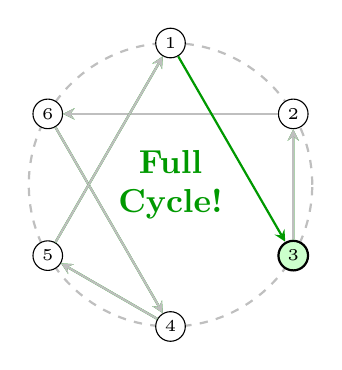
\begin{tikzpicture}[scale=1.20, transform shape]
                % Rysowanie przerywanego okręgu
                \draw[thick, dashed, gray!50] (0,0) circle (1.5cm);
                
                % Definiowanie wszystkich punktów na okręgu (białe tło)
                \foreach \x/\label in {90/1, 30/2, 330/3, 270/4, 210/5, 150/6} {
                    \node[draw, circle, fill=white, inner sep=1.5pt, font=\tiny] (N\label) at (\x:1.5cm) {\label};
                }
                
                % PODKREŚLENIE GENERATORA (g=3) od samego początku
                \node[draw, circle, fill=green!20, thick, inner sep=1.5pt, font=\tiny] (N3) at (330:1.5cm) {3};

                % Krok 2: 3 -> 2
                \draw<2>[->, thick, green!60!black, >=stealth] (N3) -- (N2);
                \draw<3->[->, thick, gray!50, >=stealth] (N3) -- (N2);

                % Krok 3: 2 -> 6
                \draw<3>[->, thick, green!60!black, >=stealth] (N2) -- (N6);
                \draw<4->[->, thick, gray!50, >=stealth] (N2) -- (N6);

                % Krok 4: 6 -> 4
                \draw<4>[->, thick, green!60!black, >=stealth] (N6) -- (N4);
                \draw<5->[->, thick, gray!50, >=stealth] (N6) -- (N4);

                % Krok 5: 4 -> 5
                \draw<5>[->, thick, green!60!black, >=stealth] (N4) -- (N5);
                \draw<6->[->, thick, gray!50, >=stealth] (N4) -- (N5);

                % Krok 6: 5 -> 1
                \draw<6>[->, thick, green!60!black, >=stealth] (N5) -- (N1);
                \draw<7->[->, thick, gray!50, >=stealth] (N5) -- (N1);

                % Krok 7: 1 -> 3 (Zamknięcie cyklu na stałe na zielono)
                \draw<7->[->, thick, green!60!black, >=stealth] (N1) -- (N3);

                % Napis pojawiający się w środku zegara na samym końcu
                \node<7-> at (0,0) [align=center, text=green!60!black] {\textbf{Full} \\ \textbf{Cycle!}};
            \end{tikzpicture}
        \end{column}
    \end{columns}
\end{frame}

\begin{frame}{The Quest for a "Good" Generator}
    
    \begin{block}{The Core Engine of Cryptography}
        Repeated modular multiplication and exponentiation are computed \textbf{constantly} in modern cryptography (e.g., the ElGamal scheme).
    \end{block}

    \vspace{0.4cm}
    \textbf{What makes a generator "Good"?}
    \begin{itemize}
        \item We want to choose a base number (generator $g$) that visits \textbf{as many points as possible} before returning to 1.
        \vspace{0.2cm}
        \item Ideally, it should visit \textit{every single valid number} in our modulo group.
        \vspace{0.3cm}
    \end{itemize}
\end{frame}

\begin{frame}{Visualizing Generators: A "Bad" Generator}
    
    \begin{block}{Repeated Multiplication (Modulo 7)}
        Now, let's see what happens if we choose number 2 as our generator instead.
    \end{block}

    \vspace{0.3cm}
    \begin{columns}[c]
        % Lewa kolumna z obliczeniami krok po kroku
        \begin{column}{0.55\textwidth}
            \begin{itemize}
                \item<1-> $2^1 \equiv \mathbf{2} \pmod 7$
                \vspace{0.1cm}
                \item<2-> $2^2 = 2^1 \cdot 2 \equiv \mathbf{2} \cdot 2 \equiv \mathbf{4} \pmod 7$
                \vspace{0.1cm}
                \item<3-> $2^3 = 2^2 \cdot 2 \equiv \mathbf{4} \cdot 2 \equiv 8 \equiv \mathbf{1} \pmod 7$
                \vspace{0.1cm}
                \item<4-> $2^4 = 2^3 \cdot 2 \equiv \mathbf{1} \cdot 2 \equiv \mathbf{2} \pmod 7$
            \end{itemize}
        \end{column}

        % Prawa kolumna z graficznym zegarem (TikZ)
        \begin{column}{0.45\textwidth}
            \centering
            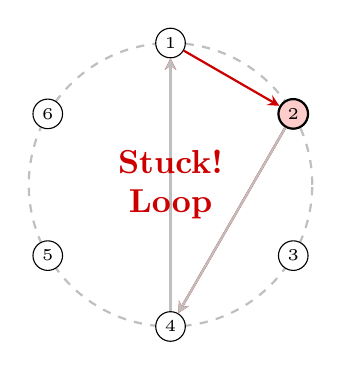
\begin{tikzpicture}[scale=1.2, transform shape]
                % Rysowanie przerywanego okręgu
                \draw[thick, dashed, gray!50] (0,0) circle (1.5cm);
                
                % Definiowanie wszystkich punktów na okręgu (białe tło)
                \foreach \x/\label in {90/1, 30/2, 330/3, 270/4, 210/5, 150/6} {
                    \node[draw, circle, fill=white, inner sep=1.5pt, font=\tiny] (N\label) at (\x:1.5cm) {\label};
                }
                
                % PODKREŚLENIE ZŁEGO GENERATORA (g=2) od samego początku
                \node[draw, circle, fill=red!20, thick, inner sep=1.5pt, font=\tiny] (N2) at (30:1.5cm) {2};

                % Krok 2: 2 -> 4
                \draw<2>[->, thick, red!80!black, >=stealth] (N2) -- (N4);
                \draw<3->[->, thick, gray!50, >=stealth] (N2) -- (N4);

                % Krok 3: 4 -> 1
                \draw<3>[->, thick, red!80!black, >=stealth] (N4) -- (N1);
                \draw<4->[->, thick, gray!50, >=stealth] (N4) -- (N1);

                % Krok 4: 1 -> 2 (Zamknięcie przedwczesnego cyklu na stałe na czerwono)
                \draw<4->[->, thick, red!80!black, >=stealth] (N1) -- (N2);

                % Napis pojawiający się w środku zegara na samym końcu
                \node<5-> at (0,0) [align=center, text=red!80!black] {\textbf{Stuck!} \\ \textbf{Loop}};
            \end{tikzpicture}
        \end{column}
    \end{columns}
\end{frame}
\begin{frame}{The Core of Security: Discrete Logarithm Problem}
    
    \begin{block}{The Trapdoor Function (One-Way Street)}
        In modular arithmetic, the equation \textbf{$y \equiv g^x \pmod p$} is easy to compute in one direction, but practically impossible to reverse. \\
        \vspace{0.1cm}
        \textit{The upcoming \textbf{ElGamal cipher} is built entirely on this mathematical foundation!}
    \end{block}

    \vspace{0.4cm}
    \begin{center}
        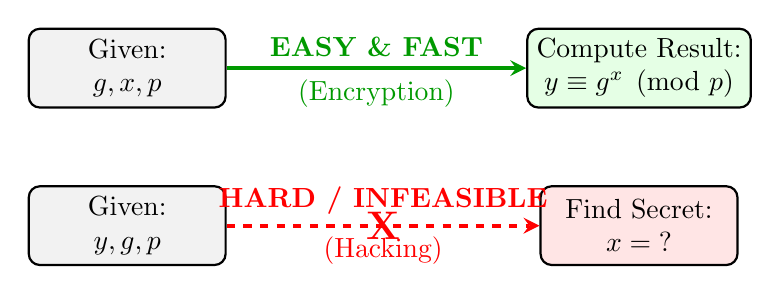
\begin{tikzpicture}[scale=1.0, transform shape, node distance=3cm]
            
            % --- EASY PATH (Encryption) ---
            \node[draw, thick, fill=gray!10, rounded corners, align=center, minimum width=2.5cm, minimum height=1cm] (A) at (0, 1.5) {Given:\\ $g, x, p$};
            
            \node[draw, thick, fill=green!10, rounded corners, align=center, minimum width=2.5cm, minimum height=1cm] (B) at (6.5, 1.5) {Compute Result:\\ $y \equiv g^x \pmod p$};
            
            \draw[->, line width=1.5pt, green!60!black, >=stealth] (A) -- (B) node[midway, above] {\textbf{EASY \& FAST}} node[midway, below] {(Encryption)};

            % --- HARD PATH (Hacking) ---
            \node[draw, thick, fill=gray!10, rounded corners, align=center, minimum width=2.5cm, minimum height=1cm] (C) at (0, -0.5) {Given:\\ $y, g, p$};
            
            \node[draw, thick, fill=red!10, rounded corners, align=center, minimum width=2.5cm, minimum height=1cm] (D) at (6.5, -0.5) {Find Secret:\\ $x = \text{?}$};
            
            \draw[->, line width=1.5pt, red, dashed, >=stealth] (C) -- (D) node[midway, above] {\textbf{HARD / INFEASIBLE}} node[midway, below] {(Hacking)};
            
            % Czerwony "X" na dolnej strzałce dla dodatkowego efektu wizualnego
            \node[text=red, font=\Large] at (3.25, -0.5) {\textbf{X}};
            
        \end{tikzpicture}
    \end{center}
    
\end{frame}

\begin{frame}{Be Careful: The Illusion of Security}
    
    \begin{alertblock}{Math is only as strong as its parameters!}
        Cryptography is secure \textbf{only if} we choose:
        \begin{itemize}
            \item Sufficiently large numbers (modulus).
            \item Proper cryptographic parameters.
            \item A "good" generator (Primitive Root).
        \end{itemize}
    \end{alertblock}

    \vspace{0.4cm}
    \textbf{What happens if we ignore this?}
    \begin{itemize}
        \item If we pick a bad generator the cycle is incredibly small (only 3 elements).
        \vspace{0.2cm}
        \item The Discrete Logarithm Problem (DLP) completely loses its "one-way" property.
        \vspace{0.2cm}
        \item An attacker can easily guess the secret exponent $x$ using simple \textbf{trial and error} (brute force)!
    \end{itemize}
\end{frame}  

\begin{frame}{The Danger of a "Bad" Generator: Brute Force Attack}
    
    \textbf{Scenario:} A hacker intercepts ciphertext $y=4$ and knows public parameters $g=2, p=7$. They want to find the secret $x$ in $2^x \equiv 4 \pmod 7$.

    \vspace{0.6cm}
    \begin{center}
        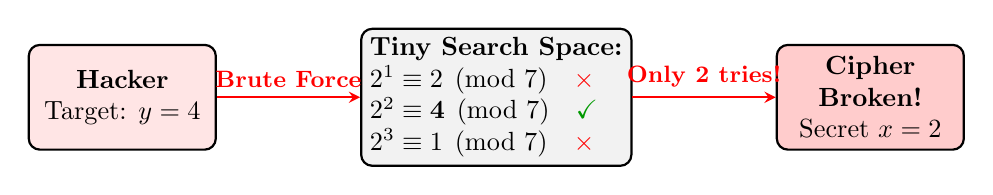
\begin{tikzpicture}[scale=0.95, transform shape]
            
            % Krok 1: Haker i jego cel
            \node[draw, thick, fill=red!10, rounded corners, align=center, minimum width=2.5cm, minimum height=1.4cm] (hacker) at (0,0) {\textbf{Hacker}\\ Target: $y=4$};
            
            % Krok 2: Przestrzeń poszukiwań (Brute Force)
            \node[draw, thick, fill=gray!10, rounded corners, align=left, minimum width=3.5cm, minimum height=1.4cm] (bruteforce) at (5,0) {
                \textbf{Tiny Search Space:} \\
                $2^1 \equiv 2 \pmod 7$ \ \ \textcolor{red}{$\times$} \\
                $2^2 \equiv \mathbf{4} \pmod 7$ \ \ \textcolor{green!60!black}{\textbf{\checkmark}} \\
                $2^3 \equiv 1 \pmod 7$ \ \ \textcolor{red}{$\times$}
            };
            
            % Krok 3: Złamany szyfr
            \node[draw, thick, fill=red!20, rounded corners, align=center, minimum width=2.5cm, minimum height=1.4cm] (broken) at (10,0) {\textbf{Cipher}\\ \textbf{Broken!} \\ Secret $x=2$};
            
            % Strzałki z opisami
            \draw[->, thick, red, >=stealth] (hacker) -- (bruteforce) node[midway, above, font=\small] {\textbf{Brute Force}};
            \draw[->, thick, red, >=stealth] (bruteforce) -- (broken) node[midway, above, font=\small] {\textbf{Only 2 tries!}};
            
        \end{tikzpicture}
    \end{center}

    \vspace{0.8cm}
    \begin{center}
        \textbf{\textit{A small subgroup completely destroys the "one-way" property of the DLP!}}
    \end{center}
\end{frame}

\section{Introduction to the ElGamal Scheme}
% Slajd 10: Wprowadzenie do algorytmu ElGamal (Kryptografia Asymetryczna)

% Slajd 10: Wprowadzenie do algorytmu ElGamal (Kryptografia Asymetryczna)
\begin{frame}{Asymmetric Cryptography: Visual Concept}
    \begin{center}
    \resizebox{0.95\textwidth}{!}{
    \begin{tikzpicture}[
        node distance=1.5cm and 2.8cm,
        box/.style={draw, thick, rounded corners, fill=blue!5, text width=4.8cm, align=center, minimum height=1.5cm},
        highlight/.style={draw, thick, rounded corners, fill=purple!5, text width=4.8cm, align=center, minimum height=1.5cm},
        arrow/.style={->, thick, >=stealth} 
    ]

    % Krok 1 (Pojawia się od razu)
    \node[highlight] (alice1) {
        \textbf{1. Alice (Receiver)}\\
        Generates key pair:\\
        \vspace{0.1cm}
        \textcolor{green!50!black}{\textbf{Public Key ($h$)}}\\
        \textcolor{red}{\textbf{Private Key ($x$)}}
    };

    % Krok 2 (Pojawia się na 2. kliknięciu)
    \uncover<2->{
        \node[box, right=2.8cm of alice1] (bob) {
            \textbf{2. Bob (Sender)}\\
            Encrypts his message using the\\
            \textcolor{green!50!black}{\textbf{Public Key ($h$)}}\\
            received from Alice.
        };
        
        % Strzałka od Alice 1 do Boba
        \only<2>{\draw[arrow, green!60!black] (alice1.east) -- node[above, align=center, text=black, font=\small] {Sends\\Public Key $h$} (bob.west);}
        \only<3->{\draw[arrow, black] (alice1.east) -- node[above, align=center, text=black, font=\small] {Sends\\Public Key $h$} (bob.west);}
    }

    % Krok 3 (Pojawia się na 3. kliknięciu)
    \uncover<3->{
        % Zmniejszono odstęp pionowy z 1.5cm na 0.6cm, aby kafelek był wyżej
        \node[highlight, below=0.6cm of alice1] (alice2) {
            \textbf{3. Alice (Receiver)}\\
            Uses her secret\\
            \textcolor{red}{\textbf{Private Key ($x$)}}\\
            to decrypt the received\\
            encrypted message.
        };
        
        % Załamana strzałka od Boba bezpośrednio do Alice 2
        \only<3>{\draw[arrow, green!60!black] (bob.south) |- node[near start, right, align=center, text=black, font=\small] {Sends\\encrypted message} (alice2.east);}
        \only<4->{\draw[arrow, black] (bob.south) |- node[near start, right, align=center, text=black, font=\small] {Sends\\encrypted message} (alice2.east);}
    }

    \end{tikzpicture}
    }
    \end{center}
\end{frame}

% Slajd 10a: Wprowadzenie do algorytmu ElGamal (Mechanika)
\begin{frame}{Historical Homomorphism: The ElGamal Scheme}
    \begin{block}{1. Key Generation}
        \begin{itemize}
            \item Choose a large prime number $p$ and a generator $g$.
            \item Choose a random private key $x$.
            \item Compute public key $h \equiv g^x \pmod p$.
        \end{itemize}
    \end{block}
    
    \vspace{0.2cm}
    \begin{columns}
        \begin{column}{0.4\textwidth}
            \begin{block}{2. Encryption}
                Message $m$. Choose random $y$.\\
                \vspace{0.1cm}
                Compute ciphertext $C = (c_1, c_2)$:
                \begin{itemize}
                    \item $c_1 \equiv g^y \pmod p$
                    \item $c_2 \equiv m \cdot h^y \pmod p$
                \end{itemize}
            \end{block}
        \end{column}
        \begin{column}{0.4\textwidth}
            \begin{block}{3. Decryption}
                Given $C = (c_1, c_2)$ and private key $x$:\\
                \vspace{0.1cm}
                Recover message $m$:
                \begin{itemize}
                    \item $s \equiv c_1^x \pmod p$
                    \item $m \equiv c_2 \cdot s^{-1} \pmod p$
                \end{itemize}
            \end{block}
        \end{column}
    \end{columns}
\end{frame}

% Slajd 10b: Przykład liczbowy ElGamal - Generacja Kluczy
\begin{frame}{ElGamal Toy Example (1/3): Key Generation}
    \textbf{Setup:} We use our "good" generator $g=3$ in $\mathbb{Z}_7^*$ (modulus $p=7$).
    
    \vspace{0.3cm}
    \begin{block}{Step 1: Receiver generates keys}
        \begin{itemize}
            \item \textbf{Private Key ($x$):} Choose a random number, e.g., $x = 2$.
            \vspace{0.2cm}
            \item \textbf{Public Key ($h$):} Compute $h \equiv g^x \pmod p \equiv \textbf{3}^{\textbf{2}} \pmod 7 = 9 \equiv \textbf{2}$
        \end{itemize}
    \end{block}
    
    \vspace{0.3cm}
    \textbf{Result:} The Receiver publicly shares $(p=7, g=3, h=2)$ and keeps $x=2$ secret.
\end{frame}

% Slajd 10c: Przykład liczbowy ElGamal - Szyfrowanie
\begin{frame}{ElGamal Toy Example (2/3): Encryption}
    \textbf{Scenario:} Sender wants to encrypt the message $m = 5$ with $(p=7, g=3, h=2)$.
    
    \vspace{0.3cm}
    \begin{block}{Step 2: Sender encrypts the message}
        \begin{itemize}
            \item \textbf{Random Element ($y$):} Choose a temporary random number, e.g., $y = 4$.
            \vspace{0.1cm}
            \item \textbf{Compute $c_1$ (Masked Key):} 
            \begin{center}
            $c_1 \equiv g^y \pmod p$
            \end{center}
            \begin{center}
                $c_1 \equiv \textbf{3}^{\textbf{4}} \equiv  81 \equiv \textbf{4} \pmod 7$
            \end{center}
            \vspace{0.2cm}
            \item \textbf{Compute $c_2$ (Masked Message):} 
            \begin{center}
            $c_2 \equiv m \cdot h^y \pmod p$
            \end{center}
            \begin{center}
                $c_2 \equiv \textbf{5} \cdot \textbf{2}^{\textbf{4}} \equiv  5 \cdot 16 \equiv  80 \equiv \textbf{3} \pmod 7$
            \end{center}
        \end{itemize}
    \end{block}
    
    \vspace{0.1cm}
    \textbf{Result:} Sender outputs Ciphertext $C = (c_1, c_2) = (4, 3)$.
\end{frame}

% Slajd 10d: Przykład liczbowy ElGamal - Deszyfrowanie
\begin{frame}{ElGamal Toy Example (3/3): Decryption}
    \textbf{Scenario:} Receiver gets Ciphertext $C = (4, 3)$ and uses Private Key $x = 2$ with $(p=7, g=3, h=2)$.
    
    \vspace{0.3cm}
    \begin{block}{Step 3: Receiver decrypts the ciphertext}
        \begin{itemize}
            \item \textbf{Recover Shared Secret ($s$):}
            \begin{center}
            $s \equiv c_1^x \pmod p$
            \end{center}
            \begin{center}
                $s \equiv \textbf{4}^{\textbf{2}} \equiv 16 \equiv \textbf{2} \pmod 7$
            \end{center}
            \vspace{0.2cm}
            \item \textbf{Recover Message ($m$):}
            \begin{center}
            $s^{-1} \equiv 2^{-1} \equiv \textbf{4} \pmod 7$                 
            \end{center}
            \begin{center}
            $m \equiv c_2 \cdot s^{-1} \pmod p$
            \end{center}
            \begin{center}
                $m \equiv \textbf{3} \cdot \textbf{4} = 12 \equiv \textbf{5} \pmod 7$
            \end{center}
        \end{itemize}
    \end{block}
\end{frame}
% Slajd 10e: Multyplikatywny homomorfizm w ElGamal (Koncepcja)
\begin{frame}{The Magic of Multiplicative Homomorphism}
    \textbf{Why ElGamal in an FHE course?} \\
    Because it natively possesses a \textit{multiplicative homomorphic} property!
    
    \vspace{0.6cm}
    This means that if we take two encrypted messages and simply multiply them together, the result is a valid ciphertext of their product. We do not need the decryption key to do this!
    
    \vspace{0.6cm}
    \begin{alertblock}{The Core Homomorphic Property}
        \begin{center}
            \Large $\text{Enc}(m_A) \cdot \text{Enc}(m_B) = \text{Enc}(m_A \cdot m_B)$
        \end{center}
    \end{alertblock}
    
    \vspace{0.6cm}
    \begin{center}
        \textit{But is this actually true? Let's prove it on the next slide!}
    \end{center}
\end{frame}

% Slajd 10f: Multyplikatywny homomorfizm w ElGamal (Dowód)
\begin{frame}{Proving the Homomorphism}
    \begin{exampleblock}{Multiplying Two Ciphertexts}
        \small
        Suppose we have two ciphertexts encrypting $m_A$ and $m_B$:
        \begin{itemize}
            \item $C_A = (c_{1A}, c_{2A}) = (g^{y_A}, \ m_A \cdot h^{y_A})$
            \item $C_B = (c_{1B}, c_{2B}) = (g^{y_B}, \ m_B \cdot h^{y_B})$
        \end{itemize}
        
        \vspace{0.2cm}
        If we multiply their components together:
        \begin{itemize}
            \item $c_{1A} \cdot c_{1B} = g^{y_A} \cdot g^{y_B} = \textbf{g}^{ \textbf{y}_A + \textbf{y}_B }$
            \item $c_{2A} \cdot c_{2B} = (m_A h^{y_A}) \cdot (m_B h^{y_B}) = \textbf{(m}_A \cdot \textbf{m}_B\textbf{)} \cdot \textbf{h}^{ \textbf{y}_A + \textbf{y}_B }$
        \end{itemize}
    \end{exampleblock}
    
    \vspace{0.2cm}
    The resulting ciphertext $(c_{1A} \cdot c_{1B}, \ c_{2A} \cdot c_{2B})$ has the exact same mathematical structure as a fresh encryption of $(m_A \cdot m_B)$ using the random value $y_A + y_B$.
\end{frame}

\section{Practical Exercises}

\begin{frame}[fragile]{Practical Exercises}
    \begin{itemize}
        \item \textbf{Task 1: Implement ElGamal Encryption Scheme in Python.} Implement key generation, encryption, and decryption.
        \item \textbf{Task 2: Design Homomorphic Encryption.} Extend the basic ElGamal scheme to demonstrate its multiplicative homomorphism.
        \item \textbf{Task 3: Implement Homomorphic Multiplication Operation.} Write a function that takes two ciphertexts as input and outputs the ciphertext of their product.
    \end{itemize}
    
    \vspace{0.3cm}
    \textbf{Bonus Tasks:}
    \begin{itemize}
        \item \textit{The Art of Generating Chaos:} Computationally find a "good" generator (a primitive root) for the group $\mathbb{Z}_p$, and intentionally select a "bad" generator to demonstrate how it fails to properly mask data.
        \item \textit{Unit Testing:} Test the implementation using \texttt{pytest}.
    \end{itemize}
\end{frame}

\end{document}